\documentclass[12pt,a4paper]{article}
\usepackage[utf8]{inputenc}
\usepackage[T1]{fontenc}
\usepackage[english]{babel}
\addto\captionsenglish{%
  \renewcommand{\contentsname}{Sumário}%
  \renewcommand{\figurename}{Figura}%
  \renewcommand{\tablename}{Tabela}%
  \renewcommand{\refname}{Referências}%
  \renewcommand{\appendixname}{Apêndice}%
}
\usepackage{amsmath,amssymb,amsfonts}
\usepackage{textcomp}
\usepackage{graphicx}
\usepackage{geometry}
\geometry{left=2.5cm,right=2.5cm,top=2cm,bottom=2cm}
\usepackage{float}
\usepackage{enumitem}
\usepackage{booktabs}
\usepackage{longtable}
\usepackage{array}
\usepackage{caption}
\usepackage[round]{natbib}
\usepackage{tikz}
\usetikzlibrary{arrows.meta,positioning,calc}
\usepackage[hidelinks]{hyperref}

\setlist{topsep=2pt,itemsep=2pt}
\renewcommand{\today}{2 de dezembro de 2026}
\graphicspath{{../figuras/}{./prints/}{./}}
\captionsetup{font=small,labelfont=bf}

\newcommand{\figprint}[3]{%
  \begin{figure}[H]\centering
  \includegraphics[width=#2\textwidth]{#1}
  \caption{#3}\label{fig:#1}\end{figure}}

% Print no visual do RStudio: editor (código do script, com número de linha) ou console (comando do script e saída do log)
\newcommand{\printr}[3]{%
  \begin{figure}[H]\centering
  \includegraphics[width=#2\textwidth]{#1}
  \caption{#3}\label{fig:#1}\end{figure}}

\begin{document}

\begin{titlepage}
  \begin{center}
    \vspace*{2cm}
    
\includegraphics[width=0.5\textwidth]{capa.jpg}\\[2.5cm]
    {\LARGE \bf Projeto B2 | Previsão do tempo de táxi\\[0.2cm] na partida em Guarulhos (SBGR)}\\[0.5cm]
    {\large TRA-48: Inteligência Analítica: Dados, Modelos e Decisões}\\[0.3cm]
    {\large Relatório de execução}\\[1.2cm]
    {\large Henri Leonardo}\\[0.3cm]
    {\large Antonio Garcia}\\[0.3cm]
    {\large Gilberto Patri}\\[1.2cm]
    {\large Profa. Mayara Condé Rocha Murça}\\[2.5cm]
    \vfill
    {\large Instituto Tecnológico de Aeronáutica}\\[0.5cm]
    {\large Divisão de Engenharia Civil-Aeronáutica}\\[0.5cm]
    {\large 2 de dezembro de 2026}
    \vfill
  \end{center}
\end{titlepage}

\tableofcontents
\newpage

%=====================================================================
\section{Problema de estudo e motivação}
%=====================================================================

O tempo de táxi na partida (\textit{taxi-out}) é o intervalo entre o \textit{pushback}, quando a aeronave deixa a posição de estacionamento, e a decolagem. Em Guarulhos, na base de janeiro de 2026 usada neste projeto, ele vai de 7 a 36 minutos, com mediana de 13,8 minutos. Essa variação não é ruído puro: depende de quantas aeronaves já estão taxiando, de qual cabeceira está em uso, do porte da aeronave e do tempo.

Saber o tempo de táxi no momento do \textit{pushback} tem uso direto na operação. Com uma boa previsão, o controle de solo consegue sequenciar as partidas e liberar o \textit{pushback} na hora certa, a companhia estima melhor o horário de decolagem e o combustível gasto em solo, e as emissões com motor ligado na pista de táxi caem. Isso impõe uma regra que atravessa o trabalho inteiro: \textbf{o modelo só pode usar o que já se sabe no momento do \textit{pushback}}.

O objetivo, conforme o enunciado do Projeto B2 \citep{enunciado}, é desenvolver um modelo preditivo do tempo de táxi na partida com métodos de aprendizado de máquina supervisionado, treinado nos 6.426 voos rotulados, e aplicá-lo aos 1.607 voos da base de teste. A submissão é avaliada pelo RMSE das previsões.

Este relatório descreve a execução completa do projeto. Todo o trabalho foi feito em R, em seis scripts que partem dos códigos dos Labs da disciplina (Seção~\ref{sec:labs}). Ao longo do texto mostramos os trechos relevantes do código, como aparecem no editor do RStudio, e as saídas do console de cada etapa, além de todos os gráficos gerados. Nos prints de console, cada comando é a linha correspondente do script e a saída é a do log de execução: 26/11 para o Script 01 (reexecutado depois da revisão descrita no Apêndice~\ref{ap:historico}), 14/11 para o Script 02 e 18/11 para os Scripts 03 a 06.

Demos peso especial às etapas anteriores aos modelos, a análise exploratória (Seção~\ref{sec:exploratoria}) e o pré-processamento (Seção~\ref{sec:preproc}), porque foram elas que definiram as variáveis, a forma de validar e boa parte das escolhas de modelagem. A Seção~\ref{sec:decisoes} organiza essas escolhas num fluxo de decisão, e cada decisão é retomada na seção em que foi tomada.

Em resumo, comparamos cinco métodos vistos na disciplina, além de duas referências simples. O modelo escolhido foi uma máquina de vetores de suporte (SVM) de regressão com kernel radial, com RMSE de 130,3~s (cerca de 2,2 minutos) na nossa base de teste interna, contra 277,0~s de quem prevê sempre a média.

%=====================================================================
\section{Decisões de projeto e fluxo de análise}\label{sec:decisoes}
%=====================================================================

\subsection{Aprofundar o conteúdo de aula}\label{sec:conteudo}

A primeira decisão de projeto foi de escopo. Em vez de procurar métodos ou técnicas de fora da disciplina, decidimos trabalhar a fundo com o que foi dado em sala, nas Aulas~1 a~6 e nos Labs~1 a~6 \citep{aulas}, e entender bem cada método antes de usá-lo. Na prática, isso significou:

\begin{itemize}
  \item \textbf{métodos}: só os vistos em aula (regressão linear, árvore, kNN, SVM e rede neural), com a teoria dos slides; ficaram de fora floresta aleatória, \textit{boosting} e outras técnicas que não foram dadas;
  \item \textbf{código}: cada etapa parte do script do Lab correspondente, com as mesmas funções e pacotes (\texttt{tree}, \texttt{caret}, \texttt{e1071}, \texttt{neuralnet}, \texttt{cluster}, \texttt{mclust}, \texttt{corrplot} e \texttt{pheatmap}), a mesma estrutura em etapas, \texttt{set.seed(1)} antes de todo sorteio e os mesmos nomes de objeto;
  \item \textbf{notação}: a dos slides; por exemplo, o custo da SVM é $\theta$ e as folgas são $\varepsilon_i$, como no slide 24 da Aula~5;
  \item \textbf{exploração e validação}: as estatísticas e gráficos da Aula~1, a partição do Lab~6, a validação cruzada da Aula~4 e os enfoques de anomalia da Aula~6;
  \item \textbf{mudanças em relação aos Labs}: só quando a execução real exigiu, sempre com o motivo registrado (Tabela~\ref{tab:mudancas}).
\end{itemize}

A motivação foi dupla. Primeiro, um método de fora traria convenções e escolhas que não discutimos em aula e que não saberíamos defender com a mesma segurança. Segundo, o problema já tinha bastante a ser explorado com as ferramentas da disciplina: a exploração rendeu as variáveis do modelo, os quatro enfoques de anomalia da Aula~6 renderam um experimento, e cada método exigiu adaptações da classificação, vista nos Labs, para a regressão.

Alguns itens não estão nos slides e foram usados porque a execução pedia. Estão listados na Tabela~\ref{tab:fora}, com o motivo de cada um; o Apêndice~\ref{ap:conceitos} relaciona todos os conceitos usados com a aula e o slide de origem.

\begin{table}[H]\centering\scriptsize
\caption{Itens usados que não estão nos slides da disciplina, e por quê.}\label{tab:fora}
\renewcommand{\arraystretch}{1.2}
\begin{tabular}{p{3.6cm}p{4.2cm}p{6.3cm}}
\toprule
Item & Onde & Motivo\\
\midrule
SVM de regressão (faixa $\varepsilon$) & M4, Seção~\ref{sec:svm} & a Aula~1 (slide 17) cita a SVM entre os métodos de classificação e regressão, mas a formulação dada (Aula~5) é a de classificação; a função \texttt{svm} do Lab~5 faz regressão quando a resposta é numérica\\
Fator de \textit{smearing} & M1, Seção~\ref{sec:m1} & consequência do log sugerido na Aula~5 (slide 52): ao voltar do log com a exponencial, a previsão fica abaixo da média\\
Coeficiente de determinação ($R^2$) & M1 & sai direto no \texttt{summary} do \texttt{lm}; estatística básica, sem uso em decisão\\
Erro padrão dos coeficientes & Interpretação & também sai no \texttt{summary} do \texttt{lm}; mostra se um efeito é distinguível de zero\\
Componentes do vento & Seção~\ref{sec:features} & a direção é um ângulo (360° = 0°); o vento calmo vem como direção 0\\
Região do destino pelo prefixo ICAO & Seção~\ref{sec:features} & o pacote \texttt{tree} aceita no máximo 32 níveis, e há 96 destinos\\
Colunas binárias (\texttt{model.matrix}) & Seção~\ref{sec:matrizes} & o kNN mede distância e a rede precisa de entradas numéricas (Aula~4, slide 16)\\
Viés (média de $\hat{y}-y$) & Resultados & mostra de que lado cada modelo erra\\
Curva suavizada no scatterplot & Figura~\ref{fig:01_08_scatter_nactive} & só guia visual (\texttt{lowess}); não entra em modelo\\
\bottomrule
\end{tabular}
\end{table}

Na revisão final, retiramos do Script 01 duas verificações que tínhamos feito e que não vêm da disciplina: um teste de Kolmogorov--Smirnov e um coeficiente de assimetria. As conclusões que elas apoiavam continuam valendo com as ferramentas da Aula~1 (Seções~\ref{sec:crwy} e~\ref{sec:descritiva}).

\subsection{Fluxo de análise e de decisão}

A Figura~\ref{fig:fluxo} mostra o caminho do dado bruto ao arquivo de submissão. Cada caixa é uma etapa; à direita está a decisão que ela produziu. Uma etapa só começava quando a anterior tinha respondido à sua pergunta, e nenhuma escolha de modelagem usou a base de teste interna, que ficou reservada para a comparação final.

\begin{figure}[H]\centering
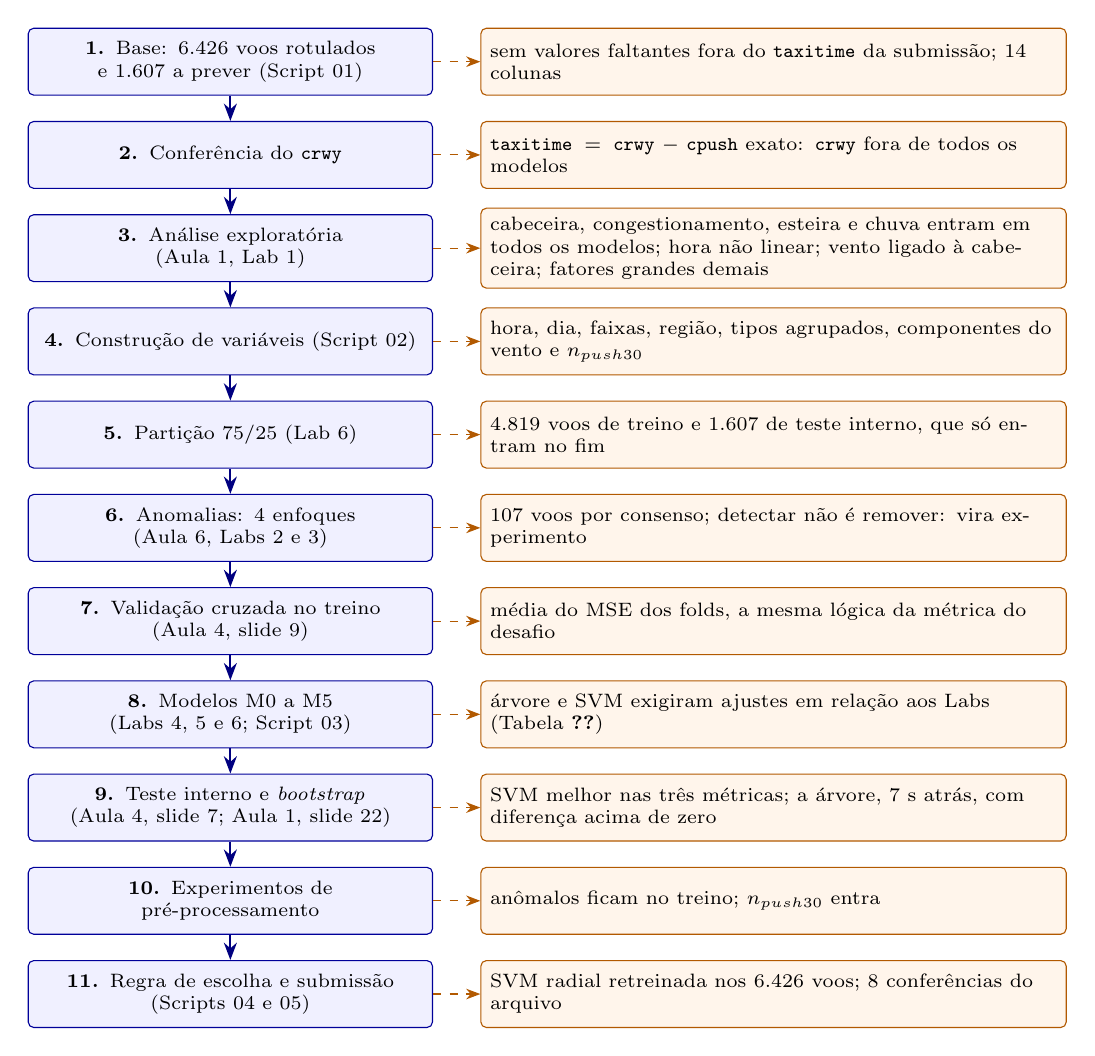
\begin{tikzpicture}[
  etapa/.style={draw=blue!60!black, fill=blue!6, rounded corners=2pt, text width=4.9cm, minimum height=0.85cm, align=center, font=\scriptsize},
  dec/.style={draw=orange!70!black, fill=orange!8, rounded corners=2pt, text width=7.2cm, minimum height=0.85cm, align=left, font=\scriptsize},
  seta/.style={-{Stealth[length=2.2mm]}, thick, blue!50!black},
  liga/.style={-{Stealth[length=1.8mm]}, dashed, orange!70!black},
  node distance=0.32cm]
\node[etapa] (e1) {\textbf{1.} Base: 6.426 voos rotulados\\e 1.607 a prever (Script 01)};
\node[etapa, below=of e1] (e2) {\textbf{2.} Conferência do \texttt{crwy}};
\node[etapa, below=of e2] (e3) {\textbf{3.} Análise exploratória\\(Aula 1, Lab 1)};
\node[etapa, below=of e3] (e4) {\textbf{4.} Construção de variáveis (Script 02)};
\node[etapa, below=of e4] (e5) {\textbf{5.} Partição 75/25 (Lab 6)};
\node[etapa, below=of e5] (e6) {\textbf{6.} Anomalias: 4 enfoques\\(Aula 6, Labs 2 e 3)};
\node[etapa, below=of e6] (e7) {\textbf{7.} Validação cruzada no treino\\(Aula 4, slide 9)};
\node[etapa, below=of e7] (e8) {\textbf{8.} Modelos M0 a M5\\(Labs 4, 5 e 6; Script 03)};
\node[etapa, below=of e8] (e9) {\textbf{9.} Teste interno e \textit{bootstrap}\\(Aula 4, slide 7; Aula 1, slide 22)};
\node[etapa, below=of e9] (e10) {\textbf{10.} Experimentos de pré-processamento};
\node[etapa, below=of e10] (e11) {\textbf{11.} Regra de escolha e submissão\\(Scripts 04 e 05)};
\foreach \a/\b in {e1/e2,e2/e3,e3/e4,e4/e5,e5/e6,e6/e7,e7/e8,e8/e9,e9/e10,e10/e11} \draw[seta] (\a) -- (\b);
\node[dec, right=0.6cm of e1] (d1) {sem valores faltantes fora do \texttt{taxitime} da submissão; 14 colunas};
\node[dec, right=0.6cm of e2] (d2) {$\texttt{taxitime}=\texttt{crwy}-\texttt{cpush}$ exato: \texttt{crwy} fora de todos os modelos};
\node[dec, right=0.6cm of e3] (d3) {cabeceira, congestionamento, esteira e chuva entram em todos os modelos; hora não linear; vento ligado à cabeceira; fatores grandes demais};
\node[dec, right=0.6cm of e4] (d4) {hora, dia, faixas, região, tipos agrupados, componentes do vento e $n_{push30}$};
\node[dec, right=0.6cm of e5] (d5) {4.819 voos de treino e 1.607 de teste interno, que só entram no fim};
\node[dec, right=0.6cm of e6] (d6) {107 voos por consenso; detectar não é remover: vira experimento};
\node[dec, right=0.6cm of e7] (d7) {média do MSE dos folds, a mesma lógica da métrica do desafio};
\node[dec, right=0.6cm of e8] (d8) {árvore e SVM exigiram ajustes em relação aos Labs (Tabela~\ref{tab:mudancas})};
\node[dec, right=0.6cm of e9] (d9) {SVM melhor nas três métricas; a árvore, 7~s atrás, com diferença acima de zero};
\node[dec, right=0.6cm of e10] (d10) {anômalos ficam no treino; $n_{push30}$ entra};
\node[dec, right=0.6cm of e11] (d11) {SVM radial retreinada nos 6.426 voos; 8 conferências do arquivo};
\foreach \i in {1,...,11} \draw[liga] (e\i) -- (d\i);
\end{tikzpicture}
\caption{Fluxo de análise: etapas (à esquerda) e a decisão que cada uma produziu (à direita).}\label{fig:fluxo}
\end{figure}

A Tabela~\ref{tab:achados} resume os achados que mais pesaram e o que cada um mudou no trabalho. Ela serve de roteiro para as Seções~\ref{sec:base} a~\ref{sec:resultados}.

\begin{table}[H]\centering\scriptsize
\caption{Achados e decisões.}\label{tab:achados}
\renewcommand{\arraystretch}{1.25}
\begin{tabular}{p{5.0cm}p{5.6cm}p{3.3cm}}
\toprule
Achado & Decisão & Onde\\
\midrule
$\texttt{taxitime}=\texttt{crwy}-\texttt{cpush}$, com o \texttt{crwy} preenchido também no teste & \texttt{crwy} fora de todos os modelos & Seção~\ref{sec:crwy}\\
cauda longa à direita (média acima da mediana; 223 voos acima do limite do boxplot) & testar a regressão linear em $\log(\texttt{taxitime})$ & Seções~\ref{sec:descritiva} e~\ref{sec:m1}\\
mediana 234~s maior na 28R & cabeceira em todos os modelos; anomalias por cabeceira & Seções~\ref{sec:categoricas} e~\ref{sec:anomalias}\\
categoria H +256~s; chuva +187~s & esteira e \texttt{wx} em todos os modelos & Seção~\ref{sec:categoricas}\\
efeito da hora sobe e desce ao longo do dia & faixas horárias na regressão; hora como número nos outros métodos & Seção~\ref{sec:hora}\\
\texttt{nactive} com $r=0{,}68$, mais inclinado na 28R & principal entrada; plano (\texttt{nactive}, \texttt{taxitime}) para as anomalias & Seção~\ref{sec:congestionamento}\\
vento correlacionado só via cabeceira; ângulo circular; calmo registrado como 0° & componentes do vento em nós & Seções~\ref{sec:correlacoes} e~\ref{sec:features}\\
96 destinos, um só no teste; tipos de aeronave com 1 a 23 voos & região do destino; tipos raros agrupados pela esteira & Seções~\ref{sec:composicao} e~\ref{sec:features}\\
PCA com variância explicada quase uniforme & sem redução de dimensão & Seção~\ref{sec:pca}\\
quatro critérios de anomalia concordam só em parte & consenso de 2 em 4; efeito de remover testado & Seções~\ref{sec:anomalias} e~\ref{sec:experimentos}\\
\texttt{cv.tree} com o mesmo erro para todos os tamanhos & validação da árvore refeita com o laço do Lab~4 & Seção~\ref{sec:arvore}\\
custo da SVM na borda da grade & grade conjunta de custo, $\gamma$ e $\varepsilon$ & Seção~\ref{sec:svm}\\
\bottomrule
\end{tabular}
\end{table}

%=====================================================================
\section{Base de dados}\label{sec:base}
%=====================================================================

A base \texttt{data\_project.Rda} traz dois objetos: \texttt{data\_train}, com 6.426 voos e o \texttt{taxitime} observado, e \texttt{data\_test}, com 1.607 voos e o \texttt{taxitime} em branco. São voos regulares partindo de Guarulhos entre 1º e 31 de janeiro de 2026. Cada linha é um voo, e as duas bases têm as mesmas 14 colunas (Figura~\ref{fig:rs_01_base_con}). A Tabela~\ref{tab:variaveis} resume as variáveis, com a definição do apêndice do enunciado e a forma como os dados se distribuem na base de treino.

\begin{table}[H]\centering\scriptsize
\caption{Variáveis da base original (valores da base de treino).}\label{tab:variaveis}
\begin{tabular}{p{2.6cm}p{5.3cm}p{6.2cm}}
\toprule
Variável & Descrição (enunciado) & Na base\\
\midrule
\texttt{id} & identificador único do voo & texto de 36 caracteres, um por voo\\
\texttt{airline} & companhia aérea (código ICAO) & 10 companhias; TAM 3.520, GLO 1.835 e AZU 448 voos (90\%)\\
\texttt{adep} & aeroporto de origem (ICAO) & sempre SBGR\\
\texttt{ades} & aeroporto de destino (ICAO) & 96 destinos; os maiores são SBRF (306), SBPA (296) e SBSV (286)\\
\texttt{acfttype} & tipo de aeronave (ICAO) & 21 tipos; A321 1.470, A320 1.442, B738 1.077, B38M 813\\
\texttt{wtc} & categoria de esteira de turbulência & H 595 e M 5.831\\
\texttt{runway} & cabeceira de decolagem & 10L 4.562 e 28R 1.864\\
\texttt{cpush} & horário do \textit{pushback} (UTC) & 01/01 a 31/01/2026\\
\texttt{crwy} & horário de decolagem (UTC) & poucos minutos depois do \texttt{cpush}\\
\texttt{taxitime} & tempo de táxi, em s (\textbf{resposta}) & 434 a 2.168~s; mediana 826,7~s\\
\texttt{nactive} & aeronaves simultaneamente em solo, em taxiamento, no momento do \textit{pushback} & 0 a 23; mediana 5\\
\texttt{wind\_direction} & direção do vento (graus) & 0 a 360°; mediana 130°\\
\texttt{wind\_speed} & velocidade do vento (kt) & 0 a 21~kt; mediana 6~kt\\
\texttt{wx} & chuva e/ou baixa visibilidade (binária) & 1 em 141 voos (2,2\%)\\
\bottomrule
\end{tabular}
\end{table}

\printr{rs_01_base_con}{0.62}{Console: formato e dimensões das duas bases (Script 01, linhas 37 a 40).}

O \texttt{summary} da base, primeiro comando do Lab~1, dá as estatísticas de todas as colunas de uma vez (Figura~\ref{fig:rs_01_sum_con}). Ele já mostra três coisas que voltam ao longo do trabalho: a cabeceira 10L concentra 71\% dos voos, a categoria H é só 9\% da amostra, e o tempo de táxi tem média (871,4~s) acima da mediana (826,7~s).

\printr{rs_01_sum_con}{0.8}{Console: \texttt{summary(data)} da base de treino (Script 01, linha 122).}

\subsection{A variável \texttt{crwy}}\label{sec:crwy}

Antes de qualquer modelo, conferimos o que a coluna \texttt{crwy} representa. O apêndice do enunciado a descreve como o horário de decolagem, e na base de treino vale exatamente
\[
\texttt{taxitime}\ [\text{s}] = \texttt{crwy} - \texttt{cpush}\ [\text{s}],
\]
com diferença máxima de zero segundo. Na base de teste o \texttt{crwy} também está preenchido. Para saber se ali ele é o horário real, comparamos o resumo (\texttt{summary}, Aula~1, slide 20) de $\texttt{crwy}-\texttt{cpush}$ no teste com o do \texttt{taxitime} do treino: mediana de 815,3~s contra 826,7~s, média de 871,9~s contra 871,4~s e quartis praticamente iguais (Figura~\ref{fig:rs_01_crwy_con}). O histograma sobreposto (Figura~\ref{fig:01_00_vazamento_crwy}) mostra a mesma forma. Ou seja, o \texttt{crwy} carrega a própria resposta nas duas bases. Como ele só existe depois da decolagem, e a previsão é feita no \textit{pushback}, usá-lo seria vazamento: o erro ficaria perto de zero no papel e o modelo não serviria na operação. Ele ficou fora de todos os modelos.

\printr{rs_01_crwy_code}{0.95}{Editor: conferência do \texttt{crwy} (Script 01, linhas 89 a 97).}
\printr{rs_01_crwy_con}{0.85}{Console: diferença máxima entre $\texttt{crwy}-\texttt{cpush}$ e \texttt{taxitime} no treino, valores faltantes do \texttt{crwy} no teste e resumo das duas distribuições.}

\figprint{01_00_vazamento_crwy}{0.85}{À esquerda, \texttt{taxitime} contra $\texttt{crwy}-\texttt{cpush}$ na base de treino. À direita, a distribuição de $\texttt{crwy}-\texttt{cpush}$ na base de teste sobre o histograma do \texttt{taxitime} do treino.}

%=====================================================================
\section{Análise exploratória}\label{sec:exploratoria}
%=====================================================================

O Script 01 segue a estrutura do \texttt{TRA48\_Lab1.R}: estatísticas descritivas (Etapa~1), visualizações gráficas (Etapa~2) e PCA (Etapa~3), com as mesmas funções (\texttt{summary}, \texttt{apply}, \texttt{aggregate}, \texttt{barplot}, \texttt{hist}, \texttt{boxplot}, \texttt{plot}, \texttt{pairs}, \texttt{corrplot}, \texttt{pheatmap} e \texttt{prcomp}). A pergunta que guiou a exploração foi prática: \textit{o que, entre as informações disponíveis no pushback, muda o tempo de táxi, e de que forma?} A resposta definiu as entradas dos modelos e a forma de cada uma.

\subsection{Estatísticas descritivas}\label{sec:descritiva}

A Tabela~\ref{tab:descritiva} traz as estatísticas do tempo de táxi, no geral e por cabeceira, calculadas como no Lab~1 (\texttt{apply} com \texttt{mean} e \texttt{var}; o desvio padrão é a raiz da variância).

\begin{table}[H]\centering\small
\caption{Estatísticas do tempo de táxi (s), geral e por cabeceira.}\label{tab:descritiva}
\begin{tabular}{lrrrrrrrr}
\toprule
Grupo & $n$ & Média & Mediana & Desvio padrão & Mín. & $Q_1$ & $Q_3$ & Máx.\\
\midrule
Geral & 6.426 & 871,4 & 826,7 & 271,2 & 434,0 & 678,5 & 1.003,3 & 2.167,9\\
10L & 4.562 & 788,6 & 751,5 & 210,6 & 434,0 & 631,3 & 909,7 & 1.736,4\\
28R & 1.864 & 1.074,2 & 985,5 & 295,2 & 599,3 & 865,4 & 1.220,8 & 2.167,9\\
\bottomrule
\end{tabular}
\end{table}

A variância é $s^2=73.555$~s$^2$ e o desvio padrão, $s=\sqrt{73.555~\text{s}^2}=271{,}2$~s, cerca de 31\% da média. A distribuição tem cauda longa à direita: a média fica acima da mediana, e a regra do boxplot (Aula~1, slide 27) marca muitos voos acima do limite superior,
\[
L = Q_3 + 1{,}5\,\text{IQR} = 1.003{,}3 + 1{,}5\times(1.003{,}3-678{,}5) = 1.003{,}3 + 1{,}5\times 324{,}8 = 1.490{,}5\ \text{s},
\]
com $Q_1$, $Q_3$ e o intervalo interquartil $\text{IQR}=Q_3-Q_1$ em segundos. São 223 voos acima de $L$ (3,5\% da base), e nenhum abaixo de $Q_1-1{,}5\,\text{IQR}=191{,}3$~s, já que o menor tempo é 434~s. A cauda está só de um lado: poucos voos demoram muito mais que o típico, e nenhum demora muito menos. O histograma em escala logarítmica fica bem mais simétrico (Figura~\ref{fig:01_01_histograma_taxitime}). Foi esse o motivo para testar a regressão linear também com $\log(\texttt{taxitime})$, que é a transformação sugerida na Aula~5 (slide 52) para tornar um modelo linear aplicável.

As duas cabeceiras já aparecem muito diferentes na própria tabela: a 28R tem média 286~s maior e desvio padrão 40\% maior que a 10L, e o voo mais longo da base está nela.

\printr{rs_01_desc_code}{0.95}{Editor: média, variância e desvio padrão (como no Lab~1) e regra do boxplot (Script 01, linhas 121 a 128 e 167 a 169).}
\printr{rs_01_desc_con}{0.7}{Console: média, variância e desvio padrão das variáveis numéricas, tabela descritiva do tempo de táxi, média e mediana e número de voos acima de $Q_3+1{,}5\,\text{IQR}$.}

\figprint{01_01_histograma_taxitime}{0.85}{Histograma do tempo de táxi e do seu logaritmo. A linha tracejada é a mediana.}
\figprint{01_02_boxplot_taxitime}{0.45}{Boxplot do tempo de táxi, com os 223 voos acima de $Q_3+1{,}5\,\text{IQR}$.}
\printr{rs_01_graf_code}{0.95}{Editor: histogramas e boxplot do tempo de táxi (Script 01, linhas 177 a 197).}

\subsection{Composição da amostra}\label{sec:composicao}

A Figura~\ref{fig:01_03_barplots_amostra} mostra como a amostra se distribui entre as categorias. TAM, GOL e Azul somam 5.803 voos, 90\% da base; a 10L recebe 71\% das partidas; e a categoria M é 91\% da amostra. Há voos em todas as horas do dia, com menos movimento na madrugada.

\figprint{01_03_barplots_amostra}{0.8}{Barplots: voos por companhia, cabeceira, categoria de esteira e hora local.}

Os fatores são grandes (Figura~\ref{fig:rs_01_lev_con}): 10 companhias, 96 destinos e 21 tipos de aeronave. Três detalhes pesaram no pré-processamento:
\begin{itemize}
  \item o destino tem 96 níveis, e o pacote \texttt{tree}, usado no Lab~4, aceita no máximo 32 por fator;
  \item o destino SDSC aparece na base de teste e não aparece na de treino, então um modelo com o destino cru não saberia prever esse voo;
  \item vários tipos de aeronave têm pouquíssimos voos: o B763 tem 1, o B737 11, o B78X 14, o B764 e o B788 20 cada, e o B77L 23. Um coeficiente estimado com um ou dois voos não generaliza.
\end{itemize}

\printr{rs_01_lev_con}{0.95}{Console: número de níveis dos fatores, destinos e tipos que só aparecem no teste e frequência dos tipos de aeronave (Script 01, linhas 141 a 144).}

\subsection{Variáveis categóricas}\label{sec:categoricas}

A cabeceira é a variável categórica de maior efeito (Figura~\ref{fig:01_04_boxplot_runway}): a mediana na 28R é 234~s maior que na 10L, quase 4 minutos. 10L e 28R são as duas pontas da mesma pista, usada em sentidos opostos; quem decide o sentido é o vento. A explicação mais provável para a diferença é a distância de táxi até a cabeceira 28R, maior para a maior parte das posições de estacionamento, mas a base não traz a posição, então isso fica como hipótese.

Aeronaves da categoria H taxiam mais que as M (medianas de 1.060~s e 804~s, +256~s), e os voos com chuva ou baixa visibilidade também (1.011~s contra 824~s, +187~s), mesmo sendo só 141 voos com $\texttt{wx}=1$ (Figura~\ref{fig:01_05_boxplot_wtc_wx}). As três variáveis entraram em todos os modelos.

\figprint{01_04_boxplot_runway}{0.7}{Tempo de táxi por cabeceira, com a mediana de cada uma.}
\figprint{01_05_boxplot_wtc_wx}{0.85}{Tempo de táxi por categoria de esteira e por condição meteorológica.}
\printr{rs_01_box_code}{0.95}{Editor: boxplots por cabeceira, por categoria de esteira e por \texttt{wx} (Script 01, linhas 216 a 236).}
\printr{rs_01_med_con}{0.45}{Console: medianas por cabeceira, categoria de esteira e \texttt{wx} (\texttt{aggregate}, como no Lab~1).}

Por companhia, a mediana vai de 696~s (ARG) a 1.113~s (AAL) (Figura~\ref{fig:01_06_boxplot_airline}). As companhias estrangeiras de longo curso (AAL, UAL, THY e QTR) ficam no alto, acima de 950~s, e as três nacionais, entre 778~s e 823~s. Boa parte dessa diferença deve vir do tipo de aeronave e do destino, e não da companhia em si: os voos de longo curso usam aeronaves H e saem para o exterior. Por isso a companhia entrou nos modelos junto com o tipo de aeronave e a região, para que cada efeito fosse separado dos demais.

\figprint{01_06_boxplot_airline}{0.85}{Tempo de táxi por companhia, ordenado pela mediana.}

\subsection{Hora do dia}\label{sec:hora}

A hora local do \textit{pushback} tem um padrão claro, mas não linear (Figura~\ref{fig:01_07_boxplot_hora} e Figura~\ref{fig:rs_01_med2_con}). As medianas sobem à 0~h (933~s), às 9~h (932~s) e às 18~h (967~s), horários que coincidem com os bancos de partidas, e caem às 5 e 6~h (cerca de 680~s) e às 20~h (662~s). A diferença entre o pico e o vale passa de 5 minutos.

Como o tempo sobe e desce ao longo do dia, um coeficiente único para a hora, numa regressão linear, não representaria esse efeito; a correlação de Pearson da hora com o tempo de táxi é só 0,07, embora o efeito seja grande. Daí a decisão de representar a hora como faixas horárias (fator) na regressão linear, e como número nos métodos que capturam relações não lineares sozinhos (árvore, kNN, SVM e rede).

\figprint{01_07_boxplot_hora}{0.85}{Tempo de táxi por hora local do \textit{pushback}.}
\printr{rs_01_med2_con}{0.42}{Console: medianas por companhia e por hora local (Script 01, linhas 137 e 138).}

\subsection{Congestionamento}\label{sec:congestionamento}

A variável numérica mais forte é o \texttt{nactive}, o número de aeronaves taxiando no momento do \textit{pushback}, com correlação de 0,68 com o tempo de táxi (Figura~\ref{fig:01_08_scatter_nactive}). A relação é aproximadamente linear e mais inclinada na 28R: com o mesmo número de aeronaves à frente, o voo que sai pela 28R demora mais. Esse efeito combinado (a inclinação muda com a cabeceira) não aparece numa regressão linear sem termos de interação, mas é capturado naturalmente por métodos como a árvore e a SVM com kernel radial, o que ajuda a entender os resultados da Seção~\ref{sec:resultados}.

\figprint{01_08_scatter_nactive}{0.8}{Tempo de táxi contra o número de aeronaves taxiando no \textit{pushback}, por cabeceira. A curva suavizada (\texttt{lowess}) é só um guia visual.}
\printr{rs_01_scat_code}{0.95}{Editor: scatterplot do congestionamento e boxplots do vento por cabeceira (Script 01, linhas 256 a 269 e 300 a 311).}

\subsection{Correlações}\label{sec:correlacoes}

O correlograma e o heatmap (Aula~1, slides 31 e 32) usam a matriz de correlação da função \texttt{cor}, que, como no Lab~1, é a de Pearson:
\[
r = \frac{\sum_i (x_i-\bar{x})(y_i-\bar{y})}{\sqrt{\sum_i (x_i-\bar{x})^2\,\sum_i (y_i-\bar{y})^2}},
\]
adimensional, porque as unidades do numerador e do denominador se cancelam, e entre $-1$ e $1$. A Figura~\ref{fig:rs_01_cor_con} mostra a matriz. O tempo de táxi se correlaciona com o \texttt{nactive} (0,68), com a direção do vento (0,29), com o \texttt{wx} (0,14), com a velocidade do vento (0,10) e quase nada com a hora (0,07, pelo motivo da seção anterior). Entre as entradas, a maior correlação é entre direção e velocidade do vento (0,28); as demais ficam abaixo de 0,16, ou seja, as entradas numéricas são pouco redundantes.

\printr{rs_01_cor_code}{0.95}{Editor: matriz de correlação, correlograma e heatmap (Script 01, linhas 280 a 297).}
\printr{rs_01_cor_con}{0.6}{Console: matriz de correlação.}
\figprint{01_10_correlograma}{0.55}{Correlograma das variáveis numéricas (\texttt{corrplot}).}
\figprint{01_11_heatmap_correlacao}{0.55}{Heatmap da matriz de correlação (\texttt{pheatmap}).}
\figprint{01_09_pairs}{0.65}{Scatterplot array (\texttt{pairs}) das variáveis numéricas, com cor pela cabeceira.}

A correlação de 0,29 da direção do vento pedia cuidado. O vento em si não deveria atrasar o táxi; o que acontece é que a cabeceira em uso acompanha o vento, porque a aeronave decola contra ele. A mediana da direção é de 110° com a 10L e de 290° com a 28R (Figura~\ref{fig:01_12_vento_runway}), justamente os rumos das duas cabeceiras. Assim, a direção do vento carrega quase a mesma informação da cabeceira, que já está nos modelos. Há ainda dois problemas no ângulo cru: ele trata 350° e 10° como valores distantes, embora sejam ventos quase iguais, e o vento calmo vem registrado como direção 0 e velocidade 0 em 239 voos (Figura~\ref{fig:rs_01_calmo_con}), o que mistura calmaria com vento de norte. Por isso o vento entrou nos modelos como componentes vetoriais (Seção~\ref{sec:features}).

\figprint{01_12_vento_runway}{0.8}{Direção e velocidade do vento por cabeceira em uso.}
\printr{rs_01_calmo_con}{0.4}{Console: direção registrada nos 239 voos com vento calmo.}

\subsection{Análise de componentes principais}\label{sec:pca}

Por fim, fizemos a PCA do Lab~1 (Etapa~3; Aula~1, slides 40 a 43) sobre as cinco variáveis numéricas de entrada, com \texttt{prcomp(x, scale=TRUE)}. Com as variáveis padronizadas, $S$ é a matriz de correlação (adimensional), e
\[
S\,u_k = \lambda_k u_k,\qquad z_{nk}=u_k^{T}x_n,\qquad \text{PVE}_k=\frac{\lambda_k}{\sum_j \lambda_j},
\]
em que $u_k$ são os pesos da componente $k$, $\lambda_k$ a variância dos dados projetados nela e $z_{nk}$ o \textit{score} do voo $n$. A variância explicada saiu quase uniforme (27,2\%, 21,3\%, 20,2\%, 17,6\% e 13,7\%; Figura~\ref{fig:01_13_pca}): seriam precisas quatro componentes para passar de 80\%. A primeira junta as variáveis de vento e o \texttt{wx} (pesos 0,60, 0,65 e 0,42), e a segunda é sobretudo a hora (0,75). O resultado confirma o que a matriz de correlação já sugeria: as entradas numéricas são pouco redundantes entre si, então não havia ganho em reduzir dimensão antes dos modelos. A PCA ficou como ferramenta de exploração.

\printr{rs_01_pca_code}{0.95}{Editor: PCA (Script 01, linhas 319 a 329).}
\printr{rs_01_pca_con}{0.62}{Console: pesos das componentes e PVE.}
\figprint{01_13_pca}{1.0}{PVE, PVE acumulada e voos no plano PC1 $\times$ PC2, com cor pela cabeceira.}

\subsection{O que a exploração decidiu}

A exploração respondeu à pergunta do início desta seção e deixou o pré-processamento quase todo definido:
\begin{enumerate}
  \item \textbf{o que entra}: congestionamento (\texttt{nactive}), o mais forte, e cabeceira, categoria de esteira e chuva, com diferenças de 3 a 4 minutos entre as categorias; tipo de aeronave, companhia, destino e hora, com efeitos menores, mas visíveis;
  \item \textbf{o que sai}: o \texttt{crwy}, que é a própria resposta, e o \texttt{adep}, que é constante;
  \item \textbf{como entra}: a hora em faixas na regressão linear; o vento em componentes; o destino e o tipo de aeronave em grupos que o pacote \texttt{tree} aceite e que tenham voos suficientes;
  \item \textbf{o que testar}: a regressão em log, por causa da cauda; e o tratamento dos voos de táxi muito longo, que aparecem na cauda e, no scatterplot, longe da nuvem principal.
\end{enumerate}

%=====================================================================
\section{Pré-processamento}\label{sec:preproc}
%=====================================================================

O Script 02 transforma a base de acordo com o que a exploração mostrou, separa treino e teste como no Lab~6, procura anomalias com os enfoques da Aula~6 e monta as matrizes numéricas do kNN e da rede. Cada passo responde a um achado da Seção~\ref{sec:exploratoria}.

\subsection{Junção das bases e descarte de variáveis}

Para que a base de treino e a de submissão recebessem exatamente as mesmas transformações e os mesmos níveis de fator, as duas foram empilhadas (8.033 voos), transformadas uma vez e separadas de novo no fim. Sem isso, um fator criado separadamente em cada base poderia ganhar níveis em ordem diferente, e o modelo treinado numa leria errado a outra. Saíram dos modelos o \texttt{crwy} (Seção~\ref{sec:crwy}), o \texttt{adep}, que vale SBGR nos 8.033 voos, e o \texttt{id}, guardado só para montar a submissão; o \texttt{cpush} foi substituído pelas variáveis de calendário abaixo.

\printr{rs_02_junta_code}{0.95}{Editor: junção das bases e descarte de variáveis (Script 02, linhas 50 a 57 e 65 a 72).}
\printr{rs_02_junta_con}{0.4}{Console: dimensão da base empilhada, voos por origem e conferência do \texttt{adep}.}

\subsection{Construção de variáveis}\label{sec:features}

Todas as variáveis novas usam só informação disponível no momento do \textit{pushback}. A Tabela~\ref{tab:features} resume cada uma e o achado que a motivou.

\begin{table}[H]\centering\scriptsize
\caption{Variáveis construídas no Script 02.}\label{tab:features}
\begin{tabular}{p{2.6cm}p{5.6cm}p{5.8cm}}
\toprule
Variável & Como foi feita & Por quê\\
\midrule
\texttt{hora} & \texttt{cpush} convertido de UTC para a hora de São Paulo (0 a 23) & efeito da hora do dia (Seção~\ref{sec:hora})\\
\texttt{dia\_semana} & dia da semana da hora local & possível diferença entre dias\\
\texttt{faixa} & hora em 6 faixas: 0--5, 6--9, 10--13, 14--17, 18--21 e 22--23~h & a regressão linear não capta o sobe e desce da hora como número\\
\texttt{regiao}, \texttt{domestico} & destino agrupado pelo prefixo ICAO & 96 destinos; limite de 32 níveis da \texttt{tree}; SDSC só no teste\\
\texttt{acft} & tipos com menos de 30 voos agrupados em \texttt{outros\_H} ou \texttt{outros\_M} & tipos raros ou inéditos no teste\\
\texttt{vento\_ns}, \texttt{vento\_lo} & componentes norte-sul e leste-oeste do vento, em kt & ângulo circular; calmo registrado como 0°\\
$n_{push30}$ & voos com \textit{pushback} nos 30~min anteriores & segunda medida de congestionamento\\
\bottomrule
\end{tabular}
\end{table}

\textbf{Calendário.} O \texttt{cpush} está em UTC e foi convertido para a hora local de São Paulo (UTC~$-$~3). Dele saíram a hora (0 a 23), o dia da semana e, para a regressão linear, seis faixas horárias. As faixas acompanham o padrão da Figura~\ref{fig:01_07_boxplot_hora} e ficaram com 683 (0--5~h), 2.051 (6--9~h), 1.262 (10--13~h), 1.671 (14--17~h), 1.178 (18--21~h) e 1.188 voos (22--23~h), somando as duas bases.

\textbf{Região do destino.} Agrupamos os destinos pelo indicador de localidade ICAO: doméstico para os prefixos atribuídos ao Brasil (SB, SD, SI, SJ, SN, SS e SW) e, para os internacionais, pela primeira letra, em América do Sul (S), América do Norte, Central e Caribe (K, C, M e T), Europa (L e E) e outros. Na base de treino ficaram 5.097 voos domésticos, 706 para a América do Sul, 363 para a América do Norte, 198 para a Europa e 62 para outros destinos; a base de submissão tem proporções parecidas e o SDSC, que só aparecia nela, virou um voo doméstico como os outros. A Figura~\ref{fig:02_01_taxitime_por_regiao} mostra que os voos internacionais taxiam mais, o que dá sentido ao agrupamento.

\figprint{02_01_taxitime_por_regiao}{0.75}{Tempo de táxi por região do destino.}

\textbf{Tipo de aeronave.} Os seis tipos com menos de 30 voos na base rotulada (B737, B763, B764, B77L, B788 e B78X) foram agrupados pela categoria de esteira: o B737 em \texttt{outros\_M} (11 voos) e os outros cinco em \texttt{outros\_H} (78 voos). Assim um tipo raro não fica com coeficiente estimado em um ou dois voos, e um tipo inédito no teste ainda recebe previsão, pelo grupo da sua categoria. O fator caiu de 21 para 17 níveis (Figura~\ref{fig:rs_02_acft_con}).

\printr{rs_02_acft_con}{0.4}{Console: voos por tipo de aeronave depois do agrupamento, na base de submissão e na de treino.}

\textbf{Vento.} Com $V$ a velocidade (kt) e $\theta$ a direção (graus),
\[
v_{ns} = V\cos\!\left(\frac{\pi\,\theta}{180}\right),\qquad v_{lo} = V\sin\!\left(\frac{\pi\,\theta}{180}\right)\qquad [\text{kt}],
\]
em que $v_{ns}>0$ indica vento de norte e $v_{lo}>0$, vento de leste. Como o seno e o cosseno são adimensionais, as duas componentes ficam em nós. Com isso 350° e 10° viram vetores quase iguais, e o vento calmo vira $(0,0)$ sem tratamento especial.

\textbf{Pushbacks recentes.} Como segunda medida de congestionamento, contamos os voos da base com \textit{pushback} nos 30 minutos anteriores ao de cada voo:
\[
n_{push30,i} = \#\{\,j : t_i - 1800\ \text{s} < t_j < t_i\,\},
\]
com $t$ o instante do \textit{pushback} em segundos. A contagem só olha para trás, então está disponível no momento da previsão e não vaza informação. Ela usa as duas bases juntas, porque todos são voos reais do mesmo mês. Vai de 0 a 18 (mediana 7) e tem correlação de 0,58 com o \texttt{nactive}: mede algo parecido, mas não igual. Como a base é uma amostra das partidas de Guarulhos, a contagem é parcial; por isso ela não entrou direto, e sim como experimento (Seção~\ref{sec:experimentos}).

\printr{rs_02_feat_code}{1.0}{Editor: construção das variáveis (Script 02, linhas 83 a 135).}
\printr{rs_02_feat_con}{0.5}{Console: voos por faixa horária, por região (treino e submissão), tipos raros e resumo do $n_{push30}$ e da sua correlação com o \texttt{nactive}.}

Depois das transformações, a base foi separada de novo em rotulada (6.426 voos) e de submissão (1.607), com 16 colunas cada, e conferimos que não havia nenhum valor faltante fora do \texttt{taxitime} da submissão (Figura~\ref{fig:rs_02_sep_con}).

\printr{rs_02_sep_code}{0.95}{Editor: fatores e separação das bases (Script 02, linhas 139 a 150).}
\printr{rs_02_sep_con}{0.4}{Console: dimensões e contagem de valores faltantes.}

\subsection{Partição treino e teste}\label{sec:particao}

Seguindo a Etapa~1 do Lab~6, com as mesmas linhas \texttt{set.seed(1)} e \texttt{sample(1:nrow(data), 0.75*nrow(data))}, a base rotulada foi dividida em 75\% para treino (4.819 voos) e 25\% para teste interno (1.607 voos, o mesmo tamanho da base da professora). A partição preservou a distribuição da resposta: médias de 870,4~s e 874,4~s e medianas de 828,1~s e 823,7~s (Figura~\ref{fig:rs_02_part_con}).

A regra para o resto do trabalho foi a do slide 7 da Aula~4: todos os hiperparâmetros são escolhidos por validação cruzada dentro do treino, e a base de teste interna só entra na comparação final dos modelos já ajustados. Assim o erro no teste interno é uma estimativa honesta do erro na base da professora.

\printr{rs_02_part_code}{1.0}{Editor: partição treino e teste (Script 02, linhas 165 a 176; em amarelo, as linhas iguais às do Lab~6).}
\printr{rs_02_part_con}{1.0}{Console: dimensões e resumo do tempo de táxi nas duas partes.}

\subsection{Detecção de anomalias}\label{sec:anomalias}

A exploração mostrou voos com tempo de táxi muito acima do esperado para o nível de congestionamento. Para identificá-los, aplicamos os enfoques da Aula~6, com o código dos Labs~2 e~3, aos voos de treino, no plano (\texttt{nactive}, \texttt{taxitime}) padronizado. O plano foi escolhido porque o tempo de táxi só é ``anômalo'' em relação ao congestionamento: um táxi longo é normal com muitas aeronaves taxiando e estranho com poucas.

\begin{itemize}
  \item \textbf{Regra do boxplot por cabeceira} (Aula~1, slides 27 a 29): acima de $Q_3+1{,}5\,\text{IQR}$ da sua cabeceira. Por cabeceira porque a 28R é mais lenta, e uma regra única marcaria quase só voos dela. Resultado: 126 voos.
  \item \textbf{k-means} (Lab~2, Etapas 1 e 3; Aula~6, slide~13): o número de clusters saiu da silhueta média, que foi máxima em $k=2$ (0,49), com o cotovelo como apoio (Figura~\ref{fig:02_02_anomalias_cotovelo_silhouette}). Para cada voo, $r_i=d_i/\bar{d}_c$, com $d_i$ a distância do voo ao centróide do seu cluster e $\bar{d}_c$ a distância média dos voos desse cluster ao centróide; anômalo se $r_i>3$. Resultado: 21 voos.
  \item \textbf{Mistura gaussiana} (Lab~3; Aula~3; Aula~6, slide~15): $p(x)=\sum_k \omega_k\,\mathcal{N}(x;\mu_k,\Sigma_k)$, estimada pelo \texttt{Mclust}, que escolheu o modelo VVV (volume, forma e orientação livres) com sete componentes pelo BIC; anômalos são os 2,5\% de menor densidade. Resultado: 121 voos.
  \item \textbf{Clusterização hierárquica} (Lab~2, Etapa~2; Aula~6, slide~14): ligação média, 20 clusters; anômalos são os voos em clusters com menos de 1\% da base. Resultado: 161 voos.
\end{itemize}

Como as distâncias são calculadas no plano padronizado, $r_i$ e as distâncias são adimensionais.

\begin{table}[H]\centering\small
\caption{Votos dos quatro critérios de anomalia nos 4.819 voos de treino.}\label{tab:votos}
\begin{tabular}{lrrrrr}
\toprule
Número de critérios que marcaram o voo & 0 & 1 & 2 & 3 & 4\\
\midrule
Voos & 4.580 & 132 & 44 & 43 & 20\\
\bottomrule
\end{tabular}
\end{table}

Os critérios concordam só em parte (Tabela~\ref{tab:votos}): 132 voos foram marcados por um só, e apenas 20 pelos quatro. As marcações da mistura gaussiana e da hierárquica são as mais parecidas (correlação de 0,67), e o k-means é o mais diferente dos outros (0,36 a 0,41), o que faz sentido: com só dois clusters, ele mede distância ao centro de grupos grandes, enquanto a mistura e a hierárquica olham para regiões de baixa densidade e grupos pequenos. Como nenhum critério sozinho é confiável, consideramos anômalo o voo marcado por pelo menos dois: 107 voos, 2,2\% do treino (Figura~\ref{fig:02_04_anomalias_consenso}).

Detectar não significa remover. A base da professora também tem voos assim, e um modelo que nunca os viu pode errar mais justamente neles. Por isso o efeito de tirá-los do treino virou um experimento (Seção~\ref{sec:experimentos}), em vez de uma limpeza feita de antemão.

\printr{rs_02_anom_code}{0.95}{Editor: os quatro critérios e o consenso (Script 02, linhas 188 a 245).}
\printr{rs_02_anom_con}{0.7}{Console: número de voos marcados por critério, silhueta por $k$, modelo do \texttt{Mclust}, votos e concordância entre os critérios.}
\figprint{02_02_anomalias_cotovelo_silhouette}{0.8}{Cotovelo e silhueta média do k-means no plano (\texttt{nactive}, \texttt{taxitime}) padronizado.}
\figprint{02_05_anomalias_silhouette_plot}{0.65}{Silhouette plot da solução com $k=2$, como no Lab~2.}
\figprint{02_03_anomalias_criterios}{0.85}{Voos marcados por cada um dos quatro critérios.}
\figprint{02_04_anomalias_consenso}{0.8}{Voos marcados como anômalos por pelo menos dois dos quatro critérios.}

A maior parte dos 107 voos fica no alto da nuvem: tempos de táxi muito longos para o congestionamento do momento. Há também alguns voos curtos demais (perto de 550~s com 9 aeronaves taxiando) e os de congestionamento extremo, acima de 15 aeronaves, onde há poucos voos. Os do alto da nuvem são os casos em que algo que a base não registra (fila na cabeceira, espera por sequenciamento, posição de estacionamento distante) pesou mais que o número de aeronaves taxiando.

\subsection{Matrizes para o kNN e a rede neural}\label{sec:matrizes}

O kNN mede distância e a rede neural precisa de entradas numéricas, então os fatores viraram variáveis binárias (\texttt{model.matrix}), num total de 42 colunas, e cada coluna foi padronizada como no slide 16 da Aula~4,
\[
z_{im}=\frac{x_{im}-\bar{x}_m}{s_m},
\]
com $x_{im}$, $\bar{x}_m$ e $s_m$ na unidade da coluna $m$, o que deixa $z$ adimensional. A média e o desvio padrão vêm só do treino e são aplicados também ao teste. Dentro da validação cruzada do Script 03, a padronização foi refeita em cada fold, só com os folds de treino, para que o fold de validação não influenciasse a escala. A variável \texttt{domestico} ficou de fora das fórmulas porque é o próprio nível \texttt{dom} da região; repeti-la daria peso dobrado a essa informação na distância do kNN.

\printr{rs_02_mat_code}{1.0}{Editor: matrizes numéricas padronizadas e fórmula comum dos modelos (Script 02, linhas 306 a 319).}
\printr{rs_02_mat_con}{0.5}{Console: dimensões das matrizes e resumo do pré-processamento.}

\subsection{O que o pré-processamento entregou}

No fim do Script 02, os modelos tinham à disposição:
\begin{itemize}
  \item 4.819 voos de treino e 1.607 de teste interno, com a mesma distribuição da resposta;
  \item onze entradas, todas conhecidas no \textit{pushback}: \texttt{nactive}, hora (ou faixa), dia da semana, cabeceira, categoria de esteira, tipo de aeronave agrupado, companhia, região do destino, as duas componentes do vento e \texttt{wx}; e o $n_{push30}$ como candidata;
  \item a marcação de 107 voos anômalos, para o experimento;
  \item as matrizes padronizadas com 42 colunas para o kNN e a rede.
\end{itemize}

%=====================================================================
\section{Métodos e treinamento dos modelos}\label{sec:metodos}
%=====================================================================

\subsection{Códigos de referência e adaptações}\label{sec:labs}

Cada método foi implementado a partir do código do Lab em que foi visto, com as mesmas funções do R. A Tabela~\ref{tab:labs} relaciona cada etapa ao código de referência e aos slides, e a Tabela~\ref{tab:mudancas} lista o que precisou mudar em relação aos Labs e por quê. Os Labs~4, 5 e~6 tratam de classificação; quase todas as mudanças vêm da passagem para uma resposta numérica, em segundos.

\begin{table}[H]\centering\scriptsize
\caption{Códigos de referência de cada etapa.}\label{tab:labs}
\begin{tabular}{p{2.8cm}p{2.2cm}p{3.3cm}p{2.8cm}p{2.6cm}}
\toprule
Etapa & Script & Código de referência & Slides & Funções\\
\midrule
Estatísticas, gráficos e PCA & Script 01 & \texttt{TRA48\_Lab1.R}, Etapas 1 a 3 & Aula 1, slides 20 a 43 & \texttt{summary}, \texttt{boxplot}, \texttt{pairs}, \texttt{corrplot}, \texttt{prcomp}\\
Partição 75/25 & Script 02 & \texttt{TRA48\_Lab6.R}, Etapa 1 & Aula 4, slide 7 & \texttt{set.seed}, \texttt{sample}\\
Anomalias: k-means e hierárquica & Script 02 & \texttt{TRA48\_Lab2.R}, Etapas 1 a 3 & Aula 2; Aula 6, slides 12 a 14 & \texttt{kmeans}, \texttt{hclust}, \texttt{silhouette}\\
Anomalias: mistura gaussiana & Script 02 & \texttt{TRA48\_Lab3.R}, Etapa 1 & Aula 3; Aula 6, slides 8 e 15 & \texttt{Mclust}, \texttt{dens}\\
Regressão linear (M1) & Script 03 & sem Lab; laço de validação do Lab 4 & Aula 5, slides 50 a 52 & \texttt{lm}, \texttt{createFolds}\\
Árvore (M2) & Script 03 & \texttt{TRA48\_Lab4.R}, Etapa 1; \texttt{TRA48\_Lab6.R}, Etapa 2 & Aula 4, slides 19 a 28; Aula 5, slide 53 & \texttt{tree}, \texttt{cv.tree}, \texttt{prune.tree}\\
kNN (M3) & Script 03 & \texttt{TRA48\_Lab4.R}, Etapa 2 & Aula 4, slides 14 a 17; Aula 5, slide 52 & \texttt{createFolds}, \texttt{knnreg}\\
SVM (M4) & Scripts 03 e 06 & \texttt{TRA48\_Lab5.R}, Etapa 1; \texttt{TRA48\_Lab6.R}, Etapa 3 & Aula 5, slides 6 a 33; Aula 1, slide 17 & \texttt{svm}, \texttt{tune}\\
Rede neural (M5) & Script 03 & \texttt{TRA48\_Lab5.R}, Etapa 2 & Aula 5, slides 34 a 47 e 54 & \texttt{neuralnet}\\
Métricas e escolha & Scripts 04 e 05 & etapas de teste dos Labs 4 a 6 & Aula 4, slides 7, 9 e 36; Aula 1, slide 22 & \texttt{predict}, \texttt{sample}\\
\bottomrule
\end{tabular}
\end{table}

\begin{table}[H]\centering\scriptsize
\caption{O que mudou em relação aos Labs.}\label{tab:mudancas}
\begin{tabular}{p{4.1cm}p{4.1cm}p{5.9cm}}
\toprule
No Lab & No projeto & Motivo\\
\midrule
Lab 4: \texttt{tree.control(mindev=0, minsize=2, mincut=1)} & \texttt{mindev=0, minsize=10, mincut=5} & com resposta contínua a árvore passava de 30 níveis (erro \textit{maximum depth reached})\\
Lab 4: \texttt{cv.tree(K=10)} para o tamanho & laço com \texttt{createFolds}, como o do kNN do Lab 4 & a \texttt{cv.tree} recresce os folds com o controle padrão e deu 155,9~s para todos os tamanhos\\
Lab 4: \texttt{knn3} & \texttt{knnreg}, do mesmo pacote \texttt{caret} & resposta numérica: média dos $k$ vizinhos (Aula 5, slide 52)\\
Lab 4: mediana da acurácia nos folds & média do MSE nos folds (mediana também calculada) & Aula 4, slide 9, e a métrica do desafio\\
Lab 5: \texttt{tune} com \texttt{cost} e \texttt{kernel} & o mesmo \texttt{tune} e depois uma grade conjunta de $\theta$, $\gamma$ e $\varepsilon$ & o custo escolhido caiu na borda da grade; o Lab deixa $\gamma$ no padrão; $\varepsilon$ só existe na regressão\\
Lab 6: \texttt{class.weights} na SVM & não usado & só existe para classificação (classes desbalanceadas)\\
Lab 5: \texttt{neuralnet} com \texttt{linear.output=FALSE} & \texttt{linear.output=TRUE}, saída padronizada, desenho por validação & saída linear para regressão (Aula 5, slide 54) e observação do próprio Lab 5\\
\bottomrule
\end{tabular}
\end{table}

\subsection{Desenho da validação e métricas}\label{sec:validacao}

Todos os modelos usam as mesmas entradas: \texttt{nactive}, hora (ou faixa, na regressão linear), dia da semana, cabeceira, categoria de esteira, tipo de aeronave, companhia, região do destino, as duas componentes do vento e \texttt{wx}. Os hiperparâmetros foram escolhidos por validação cruzada de 10 folds (5 no kNN e na rede, pelo custo computacional), sempre dentro dos 4.819 voos de treino, com \texttt{set.seed(1)} antes de cada divisão, como no Lab~4.

Na agregação entre folds calculamos a média e a mediana do erro, e decidimos pela média do MSE. O slide 9 da Aula~4 manda escolher o modelo de menor erro médio de validação, e o RMSE do desafio é a raiz de uma média de erros quadráticos sobre todos os voos; a mediana descartaria justamente os folds com erros grandes, que são os que mais pesam nessa métrica. O código do kNN no Lab~4 usa a mediana; mostramos as duas sempre que diferem.

As métricas (Aula~4, slide 36), com $y_i$ o tempo real e $\hat{y}_i$ o previsto, ambos em segundos, são
\[
\text{RMSE} = \sqrt{\frac{1}{n}\sum_{i=1}^{n}(\hat{y}_i-y_i)^2}\ [\text{s}],\qquad
\text{MAE} = \frac{1}{n}\sum_{i=1}^{n}|\hat{y}_i-y_i|\ [\text{s}],
\]
\[
\text{MAPE} = \frac{100}{n}\sum_{i=1}^{n}\left|\frac{\hat{y}_i-y_i}{y_i}\right|\ [\%].
\]
O RMSE fica em segundos porque é a raiz de s$^2$; o MAPE é adimensional, já que a razão de dois tempos se cancela. Na validação cruzada com $K$ folds, o erro de cada configuração foi
\[
\text{RMSE}_{\text{val}} = \sqrt{\frac{1}{K}\sum_{k=1}^{K}\text{MSE}_k}\ [\text{s}],
\]
com $\text{MSE}_k$ o erro quadrático médio no fold $k$ (s$^2$). O RMSE é o critério de escolha, porque é a métrica do desafio; o MAE e o MAPE são reportados, como pede o enunciado.

\subsection{Referências simples (M0)}

Para saber se um modelo é bom, comparamos com duas previsões sem aprendizado: a média do treino para todos os voos e a mediana do treino por cabeceira (751,7~s na 10L e 990,6~s na 28R). Um modelo que não bate essas referências não está aprendendo nada útil.

\subsection{Regressão linear (M1)}\label{sec:m1}

A regressão linear da Aula~5 (slides 50 e 51), $y=w^{T}x+b$, ajustada por mínimos quadrados,
\[
E=\sum_{i=1}^{n}\left(y_i-w^{T}x_i-b\right)^2\ [\text{s}^2],
\]
com a hora em faixas. Os coeficientes $w$ ficam em segundos por unidade de cada variável, ou em segundos em relação à categoria de referência, no caso dos fatores. Por causa da cauda da Seção~\ref{sec:descritiva}, testamos também o modelo em $\log(\texttt{taxitime})$, seguindo o slide 52 da Aula~5, que sugere transformar as variáveis para que um modelo linear se torne aplicável. Ao voltar do log para segundos com a exponencial, a previsão fica abaixo da média, porque a exponencial da média do log não é a média; o fator de \textit{smearing}, média de $\exp(e_i)$, corrige isso (Tabela~\ref{tab:fora}):
\[
\hat{y}=\exp(x^{T}\hat{\beta})\cdot\frac{1}{n}\sum_i \exp(e_i),
\]
com $e_i$ os resíduos do modelo em log (adimensionais).

Na validação cruzada os RMSE foram 147,4~s (linear), 149,2~s (log) e 149,1~s (log com \textit{smearing}), e ficamos com a versão linear. O log deixa a distribuição mais simétrica, mas o RMSE é medido em segundos, e a cauda, que o log comprime, é justamente o que mais pesa nele. O ajuste da versão linear no treino tem $R^2=0{,}708$, ou seja, explica 71\% da variação do tempo de táxi, e erro padrão residual de 146,1~s. Três coeficientes não são estimáveis (\texttt{acftoutros\_H}, \texttt{airlineCMP} e \texttt{airlineGLO}), porque essas colunas são combinação linear de outras; por exemplo, algumas companhias operam um único conjunto de tipos de aeronave, e então a coluna da companhia é a soma das colunas desses tipos. O R descarta essas colunas, e as previsões não mudam.

\printr{rs_03_lm_code}{0.85}{Editor: validação cruzada das três versões da regressão (Script 03, linhas 86 a 104).}
\printr{rs_03_lm_con}{0.62}{Console: medianas por cabeceira (M0), RMSE de validação das três versões, ajuste da versão linear e termos não estimáveis.}

\subsection{Árvore de regressão (M2)}\label{sec:arvore}

Mesmo procedimento do Lab~4 e do Lab~6: crescer uma árvore grande e podar por validação cruzada. Na regressão a impureza do nó passa a ser o erro quadrático médio (Aula~5, slide 53),
\[
\text{MSE}(A)=\frac{1}{n}\sum_{i\in A}\left(y_i-\bar{y}_A\right)^2\ [\text{s}^2],
\]
e o teste $x_j<s$ escolhido em cada nó é o que minimiza $\frac{n}{N}\text{MSE}(A)+\frac{m}{N}\text{MSE}(B)$, com $n$ e $m$ os voos dos filhos $A$ e $B$ e $N=n+m$. A previsão de cada folha é a média $\bar{y}$ do tempo de táxi dos voos dela. Dois ajustes foram necessários na execução real.

O primeiro foi no controle de crescimento. Com \texttt{mindev=0, minsize=2, mincut=1}, o do Lab~4, quase toda folha só fica pura com um único voo quando a resposta é contínua, e a árvore passa de 30 níveis, o limite do pacote \texttt{tree}. Mantivemos \texttt{mindev=0} e usamos o \texttt{minsize=10} e o \texttt{mincut=5} padrão do \texttt{tree.control}, o que deu uma árvore de 756 folhas.

O segundo foi na escolha do tamanho. A função \texttt{cv.tree} devolveu exatamente o mesmo RMSE (155,9~s) para todos os tamanhos de 9 a 756 folhas, e o \texttt{which.min} ficaria com a árvore inteira só por ser a primeira do empate. Isso indica que, dentro de cada fold, a \texttt{cv.tree} cresce a árvore com o controle padrão do pacote, e não com o nosso, de modo que tamanhos maiores nunca são avaliados. Refizemos a validação como o laço do kNN no Lab~4: em cada um dos 10 folds a árvore é crescida com o mesmo controle, podada em cada tamanho e avaliada no fold de validação. O mínimo ficou em 60 folhas, com RMSE de 141,9~s (Figura~\ref{fig:03_01_arvore_validacao_cruzada}). A curva mostra o comportamento esperado da Aula~4: árvores pequenas erram por simplificar demais, e as grandes voltam a piorar porque começam a decorar o treino.

\printr{rs_03_tree_code}{1.0}{Editor: árvore com o controle ajustado e validação refeita com \texttt{createFolds} (Script 03, linhas 147 a 184; em amarelo, as linhas que mudam em relação ao Lab~4).}
\printr{rs_03_tree_con}{0.55}{Console: resumo da árvore grande, RMSE da \texttt{cv.tree} (155,9~s em 553 tamanhos), RMSE de validação por tamanho e tamanho ótimo.}

\figprint{03_01_arvore_validacao_cruzada}{0.8}{RMSE de validação cruzada da árvore por número de folhas. Em azul, a validação refeita com o mesmo controle em todos os folds; em cinza, a \texttt{cv.tree}.}

\subsection{kNN (M3)}

O kNN do Lab~4 com a função \texttt{knnreg}, versão de regressão da \texttt{knn3} no mesmo pacote \texttt{caret}: a previsão é a média do tempo de táxi dos $k$ vizinhos mais próximos (Aula~5, slide 52),
\[
\hat{y}(x) = \frac{1}{k}\sum_{i\in N_k(x)} y_i\quad[\text{s}],
\]
com $N_k(x)$ os $k$ voos de treino mais próximos de $x$, em distância euclidiana nas 42 colunas padronizadas. Testamos $k$ entre 1 e 100. A média dos folds escolheu $k=5$ (RMSE de 175,1~s) e a mediana, $k=3$ (Figura~\ref{fig:03_03_knn_validacao_cruzada}); pelo critério adotado, ficou $k=5$.

\printr{rs_03_knn_code}{0.9}{Editor: validação cruzada do kNN, com a padronização refeita em cada fold (Script 03, linhas 233 a 258).}
\printr{rs_03_knn_con}{0.75}{Console: RMSE de validação por $k$, pela média e pela mediana dos folds.}
\figprint{03_03_knn_validacao_cruzada}{0.75}{RMSE de validação cruzada do kNN por número de vizinhos.}

\subsection{SVM de regressão (M4)}\label{sec:svm}

A Aula~1 (slide 17) lista as máquinas de vetores de suporte entre os métodos de classificação e regressão, mas a formulação desenvolvida na Aula~5 (slides 6 a 33) e os Labs~5 e~6 tratam só da classificação, e a lista de métodos não lineares para regressão (Aula~5, slides 52 a 55) traz kNN, CART e redes. A mesma função \texttt{svm} do pacote \texttt{e1071}, usada no Lab~5, faz regressão quando a resposta é numérica (\textit{$\varepsilon$-regression}). Por isso a incluímos como a única extensão de método do trabalho, com a formulação de regressão tirada de \citet{drucker1997} e \citet{smola2004}. Na aula, o caso não separável é escrito (Aula~5, slide 24) como
\[
\min_{w,b,\varepsilon}\ \frac{\lVert w\rVert^2}{2} + \theta\sum_{i=1}^{n}\varepsilon_i
\quad\text{sujeito a}\quad y_i(w^{T}x_i+b)\ge 1-\varepsilon_i,\ \ \varepsilon_i\ge 0,
\]
com $\varepsilon_i$ as folgas e $\theta$ o custo (o argumento \texttt{cost} do R). Na regressão, em vez de uma margem separando duas classes, a SVM ajusta uma função $f(x)=w^{T}\phi(x)+b$ e só penaliza os pontos que ficam fora de uma faixa de meia-largura $\varepsilon$ em torno dela:
\[
\min_{w,b,\xi,\xi^*}\ \frac{\lVert w\rVert^2}{2} + \theta\sum_{i=1}^{n}(\xi_i+\xi_i^*)
\quad\text{sujeito a}\quad
y_i - f(x_i) \le \varepsilon+\xi_i,\ \ f(x_i)-y_i \le \varepsilon+\xi_i^*,\ \ \xi_i,\xi_i^*\ge 0.
\]
Aqui $\varepsilon$ é o argumento \texttt{epsilon} da função \texttt{svm}, a meia-largura da faixa, e por isso as folgas acima e abaixo dela foram chamadas de $\xi_i$ e $\xi_i^*$, para não confundir com os $\varepsilon_i$ do slide. A estrutura é a mesma do slide 24: $\lVert w\rVert^2/2$ pede uma função suave, e o custo $\theta$ pesa os erros. O kernel radial do slide 33, $K(x_i,x_j)=e^{-\gamma\lVert x_i-x_j\rVert^2}$, trata relações não lineares. A função padroniza entradas e saída internamente, então $\varepsilon$ está em desvios padrão do tempo de táxi: com o desvio de 269~s do treino, $\varepsilon=0{,}1$ equivale a uma faixa de $\pm27$~s e $\varepsilon=0{,}4$, a $\pm108$~s.

A escolha foi feita em duas etapas, as duas com \texttt{tune} (validação cruzada de 10 folds, como nos Labs 5 e 6). A primeira, igual à dos Labs, comparou os kernels linear e radial com custos de 0,1 a 100: o radial com $\theta=10$ ganhou (133,3~s), e o linear ficou em torno de 148,8~s em todos os custos. O kernel linear dá praticamente o mesmo erro da regressão linear (147,4~s), o que é coerente: os dois ajustam uma função linear das entradas, só com funções de perda diferentes. A segunda etapa refinou o kernel radial numa grade conjunta de custo (0,3 a 10), $\gamma$ (1 a 8 vezes o padrão $1/42$) e $\varepsilon$ (0,05 a 0,8), com 96 combinações, porque ajustar um parâmetro de cada vez pode deixar passar combinações melhores. O ótimo foi $\theta=3$, $\gamma=4/42\approx0{,}095$ e $\varepsilon=0{,}4$, com RMSE de validação de 131,5~s e 1.960 vetores de suporte, ou seja, 41\% dos voos de treino ficam na borda ou fora da faixa. O ótimo ficou no interior da grade nas três dimensões (Figura~\ref{fig:03_04b_svm_refinamento}).

\printr{rs_03_svm1_code}{0.95}{Editor: escolha de kernel e custo com o \texttt{tune} dos Labs 5 e 6 (Script 03, linhas 293 a 301).}
\printr{rs_03_svm1_con}{0.6}{Console: resultado do \texttt{tune} e RMSE de validação por kernel e custo.}
\figprint{03_04_svm_validacao_cruzada}{0.75}{RMSE de validação cruzada da SVM por custo, com kernel linear e radial.}
\printr{rs_03_svm2_code}{1.0}{Editor: grade conjunta de custo, $\gamma$ e $\varepsilon$, com aviso automático de ótimo na borda (Script 03, linhas 311 a 330).}
\printr{rs_03_svm2_con}{0.7}{Console: dez melhores combinações, parâmetros escolhidos e resumo do modelo (1.960 vetores de suporte).}
\figprint{03_04b_svm_refinamento}{0.8}{Refinamento da SVM: RMSE de validação cruzada por $\varepsilon$ e custo, com $\gamma=4\times$ padrão.}

As dez melhores combinações da grade ficaram todas entre 131,5~s e 132,6~s (Figura~\ref{fig:06_01_svm_sensibilidade}): o resultado não depende de um ajuste fino dos hiperparâmetros. Uma faixa mais larga que a padrão ajuda porque, com erros típicos da ordem de 100~s, ignorar desvios pequenos deixa o modelo menos sensível ao ruído dos voos individuais.

\figprint{06_01_svm_sensibilidade}{1.0}{Sensibilidade da SVM ao custo, ao $\gamma$ e ao $\varepsilon$ (validação cruzada de 10 folds).}

O Script 06 registra a versão anterior do Script 03, que refinava só o custo (1, 10 e 100) com $\varepsilon$ no padrão de 0,1 e tinha escolhido $\theta=1$, o menor valor da grade. O que motivou a revisão foi esse ótimo na borda, visível na própria validação. Essa versão dava 132,8~s na validação e 132,9~s no teste interno; com a grade conjunta, 131,5~s e 130,3~s, uma redução de 2,6~s no teste com intervalo de 95\% de 0,5 a 4,7~s (\textit{bootstrap} pareado). Os hiperparâmetros novos saíram da validação; o teste só registrou o efeito. O Script 03 foi atualizado com a grade conjunta antes da submissão.

\printr{rs_06_code}{0.9}{Editor: grade conjunta do Script 06 (linhas 63 a 81).}
\printr{rs_06_con}{0.7}{Console: parâmetros da versão anterior, meia-largura da faixa em segundos, dez melhores combinações e resumo da comparação.}

\subsection{Rede neural (M5)}

A rede do Lab~5 (\texttt{neuralnet}), com a mudança indicada no slide de redes para regressão (Aula~5, slide 54): uma camada de saída com um neurônio linear (\texttt{linear.output=TRUE}),
\[
z_j=\sum_i x_i W_{ij}+W_{0j},\qquad f(z)=\frac{1}{1+e^{-z}},\qquad \hat{y} = \sum_{j} w_j\, f(z_j) + w_0,
\]
com $f$ logística nas camadas escondidas e erro $E(w)=\frac{1}{2}\sum(y-\hat{y})^2$ minimizado por retropropagação (slides 45 a 47). As entradas foram as 42 colunas padronizadas, e a saída foi padronizada para o treino e convertida de volta para segundos na previsão. Seguindo a observação do Lab~5, o desenho da rede foi escolhido por validação cruzada de 5 folds entre uma camada com 2, 3 ou 5 neurônios e duas camadas com 5 e 3, com limiar de parada de 0,1 na derivada do erro e até $2\times10^5$ passos. Todas as configurações convergiram em todos os folds; a de 3 neurônios teve o menor erro (141,5~s, contra 146,1~s, 145,9~s e 144,2~s; Figura~\ref{fig:03_05_rede_validacao_cruzada}). Redes maiores não ajudaram: com 4.819 voos, mais pesos significam mais chance de ajustar ruído.

\printr{rs_03_nn_code}{0.95}{Editor: validação cruzada da rede neural (Script 03, linhas 401 a 445; em amarelo, a chamada com \texttt{linear.output=TRUE}).}
\printr{rs_03_nn_con}{0.85}{Console: RMSE de validação por desenho da rede e desenho escolhido.}
\figprint{03_05_rede_validacao_cruzada}{0.75}{RMSE de validação cruzada da rede neural por arquitetura.}
\figprint{03_06_rede_neural}{0.85}{Rede final, com uma camada escondida de três neurônios (função \texttt{plot}, como no Lab~5).}

\subsection{Resumo do treinamento}

\begin{table}[H]\centering\small
\caption{Hiperparâmetros escolhidos por validação cruzada e tempo de execução no Mac do grupo.}\label{tab:hiper}
\begin{tabular}{llrr}
\toprule
Modelo & Escolha & RMSE de validação (s) & Tempo (s)\\
\midrule
M1 regressão linear & versão linear, hora em faixas & 147,4 & --\\
M2 árvore & 60 folhas & 141,9 & 114\\
M3 kNN & $k=5$ & 175,1 & 8\\
M4 SVM & radial, $\theta=3$, $\gamma=0{,}095$, $\varepsilon=0{,}4$ & 131,5 & 1.606\\
M5 rede neural & 1 camada, 3 neurônios & 141,5 & 346\\
\bottomrule
\end{tabular}
\end{table}

\printr{rs_03_res_con}{0.62}{Console: hiperparâmetros escolhidos e tempo de cada etapa (s).}

Já na validação a ordem estava clara: a SVM na frente, a árvore e a rede uns 10~s atrás, a regressão linear depois e o kNN bem atrás. A SVM também foi, de longe, a mais cara: 27 minutos, contra menos de 8 minutos dos outros três somados.

%=====================================================================
\section{Resultados}\label{sec:resultados}
%=====================================================================

\subsection{Comparação na base de teste interna}

A Tabela~\ref{tab:metricas} e a Figura~\ref{fig:04_01_metricas_por_modelo} trazem as métricas dos modelos na base de teste interna, que nenhum deles viu durante o ajuste. O viés é a média de $\hat{y}-y$: positivo quando o modelo superestima, negativo quando subestima.

\begin{table}[H]\centering\small
\caption{Desempenho na base de teste interna (1.607 voos).}\label{tab:metricas}
\begin{tabular}{lrrrr}
\toprule
Modelo & RMSE (s) & MAE (s) & MAPE (\%) & Viés (s)\\
\midrule
\textbf{M4 SVM} & \textbf{130,3} & \textbf{102,3} & \textbf{12,27} & 2,7\\
M2 árvore & 137,3 & 106,5 & 12,52 & $-1{,}1$\\
M5 rede neural & 142,7 & 108,7 & 12,77 & 1,0\\
M1 regressão linear & 146,8 & 114,0 & 13,41 & 1,3\\
M1 regressão linear (log) & 150,0 & 113,2 & 13,01 & $-9{,}8$\\
M3 kNN & 171,1 & 125,5 & 14,34 & $-21{,}6$\\
M0 mediana por cabeceira & 251,3 & 185,2 & 20,52 & $-53{,}7$\\
M0 média & 277,0 & 208,8 & 25,05 & $-3{,}9$\\
\bottomrule
\end{tabular}
\end{table}

\printr{rs_04_met_code}{0.95}{Editor: cálculo das métricas (Script 04, linhas 64 a 74).}
\printr{rs_04_met_con}{0.75}{Console: métricas na base de teste interna.}
\figprint{04_01_metricas_por_modelo}{1.0}{RMSE, MAE e MAPE de cada modelo na base de teste interna.}

A SVM foi a melhor nas três métricas. A ordem dos demais pelo RMSE se repete no MAE e no MAPE, com uma exceção: a regressão em log tem RMSE maior que a linear, mas MAE e MAPE menores. Faz sentido, porque o log comprime os erros grandes no ajuste e a volta para segundos subestima a cauda (viés de $-9{,}8$~s). O kNN ficou bem atrás dos outros métodos: com 42 colunas, a maioria binária, a distância entre voos fica dominada pelos fatores, e o congestionamento pesa como uma coluna entre 42; ele também é o mais enviesado ($-21{,}6$~s). A ordem no teste interno é praticamente a da validação (só a árvore e a rede, quase empatadas na validação, trocam de lugar), e os erros ficaram próximos dos de validação, o que indica que a validação cruzada estimou bem o desempenho fora do treino.

Também vale ler a tabela de baixo para cima. Só separar por cabeceira já tira 26~s do erro da média; a regressão linear, a rede, a árvore e a SVM tiram mais 100 a 120~s. O ganho principal vem de combinar o congestionamento com a cabeceira e as demais variáveis, e não de um único fator.

Os histogramas de erro (Figura~\ref{fig:04_02_histogramas_de_erros}) confirmam a tabela: os modelos com aprendizado têm erros centrados em zero e bem mais concentrados que as referências, e a cauda à esquerda (tempo real muito maior que o previsto) é o que mais pesa no RMSE de todos eles.

\figprint{04_02_histogramas_de_erros}{1.0}{Histogramas de erro ($\hat{y}-y$) na base de teste interna.}
\figprint{04_03_boxplot_erros}{0.75}{Boxplot dos erros por modelo na base de teste interna.}

A Figura~\ref{fig:04_04_real_x_previsto} compara o tempo real com o previsto. Todos os modelos achatam os extremos: preveem o tempo médio de cada situação, e os táxis muito longos ficam acima da reta de 45°, subestimados.

\figprint{04_04_real_x_previsto}{0.9}{Tempo de táxi real contra o previsto na base de teste interna, com a reta de 45°.}

\subsection{Incerteza do RMSE}

Como a diferença entre os primeiros colocados é de poucos segundos, medimos a incerteza com a reamostragem com reposição (\textit{bootstrap}) da Aula~1, slide 22: 2.000 reamostragens dos 1.607 voos de teste, com o intervalo de 95\% dado pelos percentis 2,5\% e 97,5\% (Aula~1, slide 20). Para comparar dois modelos, reamostramos os mesmos voos para os dois e olhamos a diferença de RMSE em cada reamostragem (\textit{bootstrap} pareado):
\[
\Delta^{*}_{b} = \text{RMSE}_{j}(b) - \text{RMSE}_{\text{SVM}}(b)\ [\text{s}],\qquad b=1,\dots,2000.
\]
O pareamento importa porque os voos difíceis são difíceis para todos os modelos; sorteando os mesmos voos, essa variação comum se cancela e sobra a diferença entre os modelos. A SVM tem RMSE de 130,3~s, com intervalo de 125,2 a 135,5~s (Figura~\ref{fig:04_06_bootstrap_rmse}). Todos os outros ficam atrás com intervalo da diferença acima de zero (Tabela~\ref{tab:pareado}); o mais próximo é a árvore, 7,0~s pior.

\begin{table}[H]\centering\small
\caption{\textit{Bootstrap} pareado: quanto cada modelo erra a mais que a SVM.}\label{tab:pareado}
\begin{tabular}{lrr}
\toprule
Modelo & Diferença de RMSE (s) & IC 95\% (s)\\
\midrule
M2 árvore & 7,0 & 2,4 a 12,0\\
M5 rede neural & 12,4 & 8,1 a 16,5\\
M1 regressão linear & 16,5 & 12,2 a 20,9\\
M3 kNN & 40,8 & 32,1 a 50,2\\
\bottomrule
\end{tabular}
\end{table}

\printr{rs_04_boot_code}{1.0}{Editor: \textit{bootstrap} e comparação pareada (Script 04, linhas 175 a 189).}
\printr{rs_04_boot_con}{0.62}{Console: intervalos de 95\% do RMSE e diferenças pareadas em relação à SVM.}
\figprint{04_06_bootstrap_rmse}{0.8}{RMSE na base de teste interna com intervalo de 95\% por \textit{bootstrap}.}

\subsection{Experimentos de pré-processamento}\label{sec:experimentos}

Com a SVM e seus hiperparâmetros fixos, testamos as duas questões que o pré-processamento tinha deixado em aberto, por validação cruzada de 5 folds dentro do treino, sem usar a base de teste interna. A regra de adoção foi fixada antes de rodar: o limite inferior do intervalo de 95\% (\textit{bootstrap} pareado sobre as previsões fora do fold) da redução do RMSE tem de ser maior que zero. No experimento das anomalias, os 107 voos saem só dos folds de treino; a validação continua com eles, porque a base da professora também os tem.

\begin{table}[H]\centering\small
\caption{Experimentos de pré-processamento com a SVM (validação cruzada de 5 folds no treino).}\label{tab:experimentos}
\begin{tabular}{lrrl}
\toprule
Variante & RMSE (s) & Redução (s) e IC 95\% & Decisão\\
\midrule
Base & 132,30 & -- & --\\
Sem os 107 anômalos no treino & 140,37 & $-8{,}07$ ($-10{,}41$ a $-5{,}87$) & descartada\\
Com $n_{push30}$ & 131,14 & $1{,}16$ ($0{,}18$ a $2{,}22$) & adotada\\
\bottomrule
\end{tabular}
\end{table}

Retirar os anômalos do treino piora o modelo em 8~s. Esses voos são raros, mas existem em qualquer base nova, e um modelo que nunca os viu subestima ainda mais a cauda. O resultado confirma a decisão da Seção~\ref{sec:anomalias} de não limpar a base de antemão. Os \textit{pushbacks} recentes ajudam pouco, mas de forma consistente (o intervalo inteiro fica acima de zero), e entraram no modelo final.

\printr{rs_04_exp_code}{0.95}{Editor: experimentos de pré-processamento e regra de adoção (Script 04, linhas 260 a 330).}
\printr{rs_04_exp_con}{0.7}{Console: RMSE de validação de cada variante e intervalo da redução.}

A regra de escolha do modelo final também foi escrita no código antes de rodar a avaliação: menor RMSE no teste interno; se o \textit{bootstrap} pareado não distinguir o primeiro de outro candidato, menor MAE; persistindo o empate, o modelo mais simples de explicar. Como nenhum modelo empatou com a SVM, a regra parou no primeiro passo.

\printr{rs_04_regra_code}{1.0}{Editor: regra de escolha do modelo final (Script 04, linhas 343 a 360).}
\printr{rs_04_regra_con}{0.62}{Console: modelo final e resumo da escolha.}

\subsection{Modelo final e submissão}

O modelo final é a SVM de regressão com kernel radial, $\theta=3$, $\gamma=0{,}095$ e $\varepsilon=0{,}4$, com as entradas da Seção~\ref{sec:validacao} mais o $n_{push30}$, retreinada nos 6.426 voos rotulados. As previsões para os 1.607 voos da base de teste foram gravadas na coluna \texttt{taxitime} do objeto \texttt{data\_test} original, sem alterar as demais colunas nem a ordem dos voos, no arquivo \texttt{data\_project\_test\_HenriAntonioGilberto.Rda}. Antes do envio conferimos, numa sessão nova do R, o nome do objeto, as 1.607 linhas, a ordem dos \texttt{id}, a ausência de valores faltantes e de valores negativos e que as outras 13 colunas eram idênticas às da base original.

As previsões vão de 508~s a 2.103~s, com média de 870,7~s e mediana de 831,1~s, próximas das do treino (871,4~s e 826,7~s). A cauda prevista é mais curta que a real (Figura~\ref{fig:05_01_previsoes_submissao}), o que é esperado: o modelo prevê o tempo médio de cada situação, e os táxis muito longos dependem de fatores que a base não registra. Pela estimativa da base de teste interna, o RMSE da submissão deve ficar perto de 130~s, com o intervalo do \textit{bootstrap}, de 125 a 136~s, como margem.

\printr{rs_05_ret_code}{1.0}{Editor: retreino do modelo final com os 6.426 voos e montagem do arquivo (Script 05, linhas 58 a 205).}
\printr{rs_05_conf_code}{1.0}{Editor: conferências do arquivo de submissão (Script 05, linhas 221 a 233).}
\printr{rs_05_conf_con}{0.75}{Console: dimensões da base de retreino, resumo das previsões e resultado das oito conferências.}

\figprint{05_01_previsoes_submissao}{0.85}{Previsões da submissão comparadas à distribuição real do treino, e por cabeceira.}

\subsection{Interpretação}

A SVM com kernel radial não tem coeficientes para ler, então usamos a árvore e a regressão linear, que ficaram a 7 e 17~s dela, para entender o que move o tempo de táxi.

\figprint{03_02_arvore_podada}{1.0}{Árvore de regressão podada em 12 folhas, só para leitura (a árvore usada na previsão tem 60).}

A árvore (Figura~\ref{fig:03_02_arvore_podada}) separa primeiro pelo congestionamento ($\texttt{nactive}<9{,}5$) e depois pela cabeceira; só então entram o tipo de aeronave e a hora. As folhas vão de 645~s (pouco tráfego, 10L, aeronave de corredor único, voo doméstico) a 1.732~s (mais de 15 aeronaves taxiando na 28R). É a mesma hierarquia que a exploração já sugeria.

A regressão linear (Figura~\ref{fig:04_07_efeitos_regressao_linear}) mede esses efeitos em segundos, mantidas as demais variáveis:
\begin{itemize}
  \item cada aeronave a mais taxiando no \textit{pushback} acrescenta 48,5~s (erro padrão de 0,7~s);
  \item a cabeceira 28R acrescenta 254~s em relação à 10L;
  \item chuva ou baixa visibilidade acrescentam 148~s;
  \item destinos internacionais taxiam mais que os domésticos: 48~s para a América do Sul, 88~s para a América do Norte e 115~s para a Europa;
  \item a categoria M taxia 118~s menos que a H;
  \item as faixas horárias e os dias da semana têm efeitos menores, de até 32~s, e o vento não é significativo depois que a cabeceira entra no modelo.
\end{itemize}

\figprint{04_07_efeitos_regressao_linear}{0.85}{Efeito de cada variável na regressão linear, com $\pm2$ erros padrão.}

Os efeitos da regressão são da mesma ordem das diferenças de mediana da exploração (254~s contra 234~s para a cabeceira; 148~s contra 187~s para a chuva). Não precisam coincidir: na regressão cada efeito é medido com as demais variáveis fixas, enquanto a exploração compara medianas brutas. A ausência de efeito do vento confirma a leitura da Seção~\ref{sec:correlacoes}: a correlação de 0,29 era a cabeceira aparecendo por outro caminho.

A diferença entre cabeceiras é provavelmente geométrica: a distância de táxi até a 28R é maior para a maior parte das posições de estacionamento. O efeito dos destinos internacionais deve estar ligado às posições do terminal internacional, que a base não traz; as duas hipóteses são compatíveis com os dados, mas não verificáveis só com eles.

O erro da SVM é parecido nas duas cabeceiras e cresce com o congestionamento (Figura~\ref{fig:04_05_erro_por_situacao}): com 12 ou mais aeronaves taxiando, a dispersão dos erros é a maior. É nessas situações que filas na cabeceira e esperas por sequenciamento, que o \texttt{nactive} capta só em parte, fazem mais diferença.

\figprint{04_05_erro_por_situacao}{0.85}{Erro da SVM por cabeceira e por nível de congestionamento.}

%=====================================================================
\section{Conclusões}\label{sec:conclusoes}
%=====================================================================

\subsection{O que explica o tempo de táxi}

O tempo de táxi na partida em Guarulhos é explicado principalmente pelo número de aeronaves já taxiando e pela cabeceira em uso, e em menor grau pela meteorologia, pelo porte da aeronave e pelo destino. A exploração, a árvore e a regressão contam a mesma história por caminhos diferentes:
\begin{itemize}
  \item \textbf{congestionamento}: cada aeronave a mais taxiando no \textit{pushback} soma cerca de 48~s; é a variável mais forte em todas as análises, e a árvore a usa na primeira divisão;
  \item \textbf{cabeceira}: sair pela 28R custa cerca de 4 minutos a mais, e o efeito do congestionamento é maior nela;
  \item \textbf{chuva ou baixa visibilidade}: cerca de 2,5 minutos a mais, mesmo sendo só 2\% dos voos;
  \item \textbf{porte e destino}: aeronaves H e voos internacionais taxiam mais, de cerca de 1 a 2 minutos;
  \item \textbf{hora}: o efeito existe, mas é não linear, ligado aos bancos de partidas; na regressão, com as demais variáveis fixas, as faixas horárias ficam com efeitos de até 32~s, bem menores que a diferença bruta entre as medianas por hora;
  \item \textbf{vento}: não tem efeito próprio; a correlação que aparece na exploração é a cabeceira vista por outro caminho.
\end{itemize}

\subsection{Desempenho e modelo final}

Com essas variáveis, o melhor modelo, uma SVM de regressão com kernel radial, chegou a um RMSE de 130,3~s na base de teste interna, contra 277,0~s da previsão pela média: o erro cai pela metade. O erro típico de um voo (MAE) é de 102~s, cerca de 12\% do tempo de táxi. A árvore de regressão ficou 7~s atrás, com diferença acima de zero no \textit{bootstrap} pareado, mas é o modelo que melhor explica o problema. Na prática, há uma troca entre precisão e leitura: a SVM erra menos, e a árvore mostra o porquê.

A boa posição da SVM e da árvore em relação à regressão linear é coerente com a exploração. Os efeitos se combinam (o congestionamento pesa mais na 28R; a hora sobe e desce), e métodos que capturam essas combinações sozinhos levaram vantagem sobre um modelo linear sem interações. O kNN, por outro lado, mostrou o limite de um método baseado em distância quando a maior parte das colunas é binária.

\subsection{Sobre as decisões do trabalho}

Olhando o fluxo da Figura~\ref{fig:fluxo} de trás para frente, algumas decisões foram as que mais pesaram:
\begin{itemize}
  \item \textbf{conferir as variáveis antes de modelar}: o \texttt{crwy} era a própria resposta; sem a conferência, qualquer modelo teria erro quase zero na validação e seria inútil na operação;
  \item \textbf{deixar a exploração definir as variáveis}: as faixas horárias, as componentes do vento, os agrupamentos de destino e de aeronave e o $n_{push30}$ saíram de achados concretos da Seção~\ref{sec:exploratoria};
  \item \textbf{não limpar a base de antemão}: o experimento mostrou que tirar os anômalos pioraria o modelo em 8~s;
  \item \textbf{ler a saída das funções, e não só o número final}: a \texttt{cv.tree} com o mesmo erro para todos os tamanhos e o custo da SVM na borda da grade foram percebidos lendo o console, e as duas correções melhoraram os modelos;
  \item \textbf{fixar as regras antes de olhar o resultado}: a agregação dos folds, a regra de adoção dos experimentos e a regra de escolha do modelo final foram escritas no código antes da avaliação.
\end{itemize}

A decisão de escopo da Seção~\ref{sec:conteudo}, de trabalhar a fundo com o conteúdo de aula, se mostrou suficiente para o problema. Os métodos e as ferramentas da disciplina cobriram todas as etapas, da exploração à escolha do modelo, e as mudanças necessárias foram adaptações dos Labs da classificação para a regressão. O único método fora da formulação vista em aula, a SVM de regressão, usa a mesma função do Lab~5 e foi tratado como extensão declarada. Em troca, conseguimos explicar cada escolha com a teoria dos slides, o que nos deu segurança para interpretar resultados inesperados, como os da árvore e da SVM.

\subsection{Limitações}

As principais limitações estão na base: um único mês de dados, uma amostra das partidas e nenhuma variável que descreva o caminho do táxi, como posição de estacionamento, distância até a cabeceira e fila de decolagem. O \texttt{nactive} é a única medida direta de congestionamento, e os erros maiores aparecem justamente nos horários mais congestionados. As explicações físicas para o efeito da 28R e dos destinos internacionais são hipóteses compatíveis com os dados, mas não verificáveis só com eles. Por fim, todos os modelos subestimam os táxis muito longos: eles preveem o tempo típico de cada situação, e a cauda depende de fatores fora da base.

Com os mesmos métodos, o caminho mais promissor seria acrescentar à base a posição de estacionamento e a distância de táxi até cada cabeceira, que provavelmente explicam boa parte da diferença entre 10L e 28R, e uma medida da fila na cabeceira, que é o que falta para os momentos de maior congestionamento.

\newpage
\begin{thebibliography}{9}

\bibitem[Drucker et al.(1997)]{drucker1997}
DRUCKER, H.; BURGES, C. J. C.; KAUFMAN, L.; SMOLA, A.; VAPNIK, V. Support vector regression machines. In: \textit{Advances in Neural Information Processing Systems 9}. Cambridge: MIT Press, 1997. p. 155--161.

\bibitem[Murça(2026a)]{aulas}
MURÇA, M. C. R. \textit{TRA-48: Inteligência Analítica. Aulas 1 a 6 e roteiros dos Labs 1 a 6 (2º bimestre)}. São José dos Campos: ITA, 2026. Material de aula.

\bibitem[Murça(2026b)]{enunciado}
MURÇA, M. C. R. \textit{Projeto B2}. São José dos Campos: ITA, 2026. Enunciado do projeto.

\bibitem[R Core Team(2026)]{r}
R CORE TEAM. \textit{R: a language and environment for statistical computing}. Versão 4.6. Viena: R Foundation for Statistical Computing, 2026. Pacotes usados: \texttt{tree}, \texttt{caret}, \texttt{e1071}, \texttt{neuralnet}, \texttt{cluster}, \texttt{mclust}, \texttt{corrplot} e \texttt{pheatmap}.

\bibitem[Smola e Schölkopf(2004)]{smola2004}
SMOLA, A. J.; SCHÖLKOPF, B. A tutorial on support vector regression. \textit{Statistics and Computing}, v. 14, n. 3, p. 199--222, 2004.

\end{thebibliography}

\appendix

\section{Origem de cada conceito usado}\label{ap:conceitos}

A tabela abaixo relaciona os conceitos usados no trabalho com a aula, o slide ou o Lab de onde vieram. Os itens fora dos slides estão marcados e explicados na Tabela~\ref{tab:fora}.

{\scriptsize
\begin{longtable}{p{4.6cm}p{4.6cm}p{5.0cm}}
\toprule
Conceito & Onde usamos & Origem\\
\midrule
\endfirsthead
\toprule
Conceito & Onde usamos & Origem\\
\midrule
\endhead
\bottomrule
\endfoot
Aprendizado supervisionado; problema de regressão & todo o trabalho & Aula 1, slide 10; Aula 5, slide 49\\
Média, mediana, quartis, percentis & Seções~\ref{sec:crwy} e~\ref{sec:descritiva}; IC do \textit{bootstrap} & Aula 1, slide 20; \texttt{summary}, Lab 1\\
Variância e desvio padrão & Seção~\ref{sec:descritiva} & Aula 1, slide 21; \texttt{var}, Lab 1\\
Intervalo interquartil e regra do boxplot & Seções~\ref{sec:descritiva} e~\ref{sec:anomalias} & Aula 1, slides 21 e 27 a 29\\
\textit{Bootstrap} (reamostragem com reposição) & incerteza do RMSE; experimentos & Aula 1, slide 22\\
Histograma, boxplot, barplot, scatterplot & Seção~\ref{sec:exploratoria} & Aula 1, slides 23 a 30; Lab 1\\
Correlograma, heatmap, \texttt{pairs} & Seção~\ref{sec:correlacoes} & Aula 1, slides 30 a 32; Lab 1\\
Correlação de Pearson & Seção~\ref{sec:correlacoes} & Aula 1, slide 31; \texttt{cor}, Lab 1\\
PCA e PVE & Seção~\ref{sec:pca} & Aula 1, slides 40 a 43; Lab 1, Etapa 3\\
Transformação logarítmica & M1 & Aula 5, slide 52\\
Partição treino e teste & Seção~\ref{sec:particao} & Aula 4, slide 7; Lab 6, Etapa 1\\
Validação cruzada com $K$ folds & Seção~\ref{sec:validacao} & Aula 4, slide 9; Lab 4\\
Padronização $z$ & Seção~\ref{sec:matrizes}; kNN e rede & Aula 4, slide 16\\
RMSE, MAE, MAPE & Seções~\ref{sec:validacao} e~\ref{sec:resultados} & Aula 4, slide 36\\
Sobreajuste & árvore, rede & Aula 4, slides 6, 17 e 25\\
k-means, centróide, cotovelo & Seção~\ref{sec:anomalias} & Aula 2, slides 16 a 31; Lab 2\\
Silhueta & Seção~\ref{sec:anomalias} & Aula 2, slides 49 a 51; Lab 2, Etapa 3\\
Clusterização hierárquica, ligação média & Seção~\ref{sec:anomalias} & Aula 2, slides 33 a 42; Lab 2, Etapa 2\\
Mistura gaussiana e BIC & Seção~\ref{sec:anomalias} & Aula 3, slides 2 a 9 e 33 e 34; Lab 3\\
Enfoques de anomalia (razão $r_i$, densidade, clusters pequenos) & Seção~\ref{sec:anomalias} & Aula 6, slides 8 a 15\\
Regressão linear e mínimos quadrados & M1 & Aula 5, slides 50 e 51\\
Árvore de regressão, impureza por MSE, poda & M2 & Aula 4, slides 19 a 28; Aula 5, slide 53; Labs 4 e 6\\
kNN de regressão, distância euclidiana & M3 & Aula 4, slides 14 a 17; Aula 5, slide 52; Lab 4\\
SVM: margem, folgas $\varepsilon_i$, custo $\theta$, vetores de suporte & M4 & Aula 5, slides 10 a 26; Lab 5\\
Kernel radial e $\gamma$ & M4 & Aula 5, slides 31 a 33\\
SVM de regressão (faixa $\varepsilon$, folgas $\xi$) & M4 & \textbf{fora dos slides}; citada na Aula 1, slide 17\\
Rede neural, função logística, retropropagação & M5 & Aula 5, slides 34 a 47\\
Saída linear para regressão & M5 & Aula 5, slide 54\\
Fator de \textit{smearing} & M1 & \textbf{fora dos slides} (Tabela~\ref{tab:fora})\\
$R^2$ e erro padrão dos coeficientes & M1, interpretação & \textbf{fora dos slides}; saída do \texttt{summary(lm)}\\
Viés & resultados & \textbf{fora dos slides} (Tabela~\ref{tab:fora})\\
Componentes do vento; prefixo ICAO & Seção~\ref{sec:features} & \textbf{fora dos slides} (Tabela~\ref{tab:fora})\\
\end{longtable}
}

\section{Reprodução}

O código está no repositório do grupo, em seis scripts R no padrão dos Labs da disciplina, que rodam em sequência:

\begin{table}[H]\centering\footnotesize
\begin{tabular}{ll}
\toprule
Script & Conteúdo\\
\midrule
\texttt{TRA48\_B2\_01\_exploracao.R} & conferência do \texttt{crwy}, estatísticas descritivas, figuras e PCA\\
\texttt{TRA48\_B2\_02\_preprocessamento.R} & variáveis novas, partição 75/25, anomalias e padronização\\
\texttt{TRA48\_B2\_03\_modelos.R} & M0 a M5 com validação cruzada\\
\texttt{TRA48\_B2\_04\_avaliacao.R} & métricas, \textit{bootstrap}, experimentos e escolha do modelo\\
\texttt{TRA48\_B2\_05\_submissao.R} & retreino nos 6.426 voos, arquivo de submissão e conferências\\
\texttt{TRA48\_B2\_06\_sensibilidade\_svm.R} & sensibilidade da SVM a custo, $\gamma$ e $\varepsilon$\\
\bottomrule
\end{tabular}
\end{table}

A base da disciplina não está no repositório. Com ela na pasta indicada no início de cada script, o comando \texttt{make b2} roda os Scripts 01 a 05 e gera as figuras e tabelas deste relatório; a execução completa leva cerca de 35 minutos, quase todos no ajuste da SVM. Cada script grava a saída do console num log de texto em \texttt{resultados/logs/}; os prints de console deste relatório reproduzem esses logs.

\section{Histórico das execuções}\label{ap:historico}

\begin{table}[H]\centering\footnotesize
\begin{tabular}{p{2.6cm}p{2.4cm}p{5.0cm}p{3.7cm}}
\toprule
Quando & Execução & O que aconteceu & O que fizemos\\
\midrule
log de 14/11, 15:06 & Scripts 01 e 02 & exploração e pré-processamento sem erros & log do Script 02 usado neste relatório\\
1ª execução & Script 03 & árvore com o controle do Lab 4: \textit{maximum depth reached} & \texttt{minsize=10} e \texttt{mincut=5}\\
2ª execução & Script 03 & \texttt{cv.tree} com 155,9~s para todos os tamanhos & laço com \texttt{createFolds}\\
versão anterior & Script 03 & SVM com $\theta=1$, o menor valor da grade, e $\varepsilon=0{,}1$ & investigado no Script 06\\
log de 18/11, 05:36 & Script 06 & grade conjunta: 132,9 $\rightarrow$ 130,3~s no teste & Script 03 atualizado\\
log de 18/11, 06:23 & Scripts 03 a 05 & versão final; oito conferências do arquivo & submissão em 18/11\\
26/11 & Script 01 & retirados o teste de Kolmogorov--Smirnov e o coeficiente de assimetria, que não são da disciplina; a conferência do \texttt{crwy} passa a usar o \texttt{summary} e o histograma, e a cauda, a regra do boxplot & demais saídas idênticas às de 14/11; nenhum número dos modelos muda\\
\bottomrule
\end{tabular}
\end{table}

\end{document}
